%% 
%% Copyright 2007-2020 Elsevier Ltd
%% 
%% This file is part of the 'Elsarticle Bundle'.
%% ---------------------------------------------
%% 
%% It may be distributed under the conditions of the LaTeX Project Public
%% License, either version 1.2 of this license or (at your option) any
%% later version.  The latest version of this license is in
%%    http://www.latex-project.org/lppl.txt
%% and version 1.2 or later is part of all distributions of LaTeX
%% version 1999/12/01 or later.
%% 
%% The list of all files belonging to the 'Elsarticle Bundle' is
%% given in the file `manifest.txt'.
%% 
%% Template article for Elsevier's document class `elsarticle'
%% with harvard style bibliographic references

%\documentclass[preprint,12pt,authoryear]{elsarticle}

%% Use the option review to obtain double line spacing
% \documentclass[authoryear,preprint,review,12pt]{elsarticle}

\documentclass[preprint,review,12pt]{elsarticle}

%% Use the options 1p,twocolumn; 3p; 3p,twocolumn; 5p; or 5p,twocolumn
%% for a journal layout:
%% \documentclass[final,1p,times,authoryear]{elsarticle}
%% \documentclass[final,1p,times,twocolumn,authoryear]{elsarticle}
%% \documentclass[final,3p,times,authoryear]{elsarticle}
%% \documentclass[final,3p,times,twocolumn,authoryear]{elsarticle}
%% \documentclass[final,5p,times,authoryear]{elsarticle}
%%\documentclass[final,5p,times,twocolumn,authoryear]{elsarticle}

%% For including figures, graphicx.sty has been loaded in
%% elsarticle.cls. If you prefer to use the old commands
%% please give \usepackage{epsfig}

% Document Formatting and Layout
\usepackage{geometry}
\usepackage{fancyhdr}
\usepackage{titlesec}
\usepackage{float}
\usepackage{subcaption}

% Math and Symbols
\usepackage{amsmath,amsfonts,amssymb}
\usepackage{mathtools}
\usepackage{bm}
\usepackage{mathrsfs}

% Graphics and Colors
\usepackage{graphicx}
\usepackage{xcolor}
\usepackage{tikz}
\usepackage{pgfplots}

% Tables
\usepackage{tabularx}
\usepackage{multirow}
\usepackage{longtable}
\usepackage{colortbl}
\usepackage{booktabs}

% Lists and Enumerations
\usepackage{enumitem}

% Hyperlinks and References
\usepackage{hyperref}
\usepackage{cleveref}

% Bibliography
%\usepackage[backend=bibtex,style=numeric]{biblatex}
\usepackage{natbib}

% Miscellaneous
\usepackage{microtype}
\usepackage{siunitx}
\usepackage{todonotes}
\usepackage{lineno}

%\usepackage{todonotes}
\usepackage{caption}
\usepackage{subcaption}
\usepackage{lipsum}
\usepackage{xspace}
\usepackage{setspace}

% Command to highlight revised text
\newcommand{\rev}[1]{\textcolor{black}{#1}}
%\newcommand{\rev}[1]{\textcolor{red}{#1}}


%% You might want to define your own abbreviated commands for common used terms, e.g.:
\newcommand{\kms}{km\,s$^{-1}$}
\newcommand{\msun}{$M_\odot}

\journal{arXiv}
\pdfoutput=1
\pgfplotsset{compat=1.18}
\begin{document}
\linenumbers
%\modulolinenumbers[5]
\onehalfspacing

\begin{frontmatter}

%% Title, authors and addresses

%% use the tnoteref command within \title for footnotes;
%% use the tnotetext command for theassociated footnote;
%% use the fnref command within \author or \affiliation for footnotes;
%% use the fntext command for theassociated footnote;
%% use the corref command within \author for corresponding author footnotes;
%% use the cortext command for theassociated footnote;
%% use the ead command for the email address,
%% and the form \ead[url] for the home page:
%% \title{Title\tnoteref{label1}}
%% \tnotetext[label1]{}
%% \author{Name\corref{cor1}\fnref{label2}}
%% \ead{email address}
%% \ead[url]{home page}
%% \fntext[label2]{}
%% \cortext[cor1]{}
%% \affiliation{organization={},
%%            addressline={}, 
%%            city={},
%%            postcode={}, 
%%            state={},
%%            country={}}
%% \fntext[label3]{}
\title{Uncertainty Quantification of Acoustic Metamaterial Bandgaps with Stochastic Material Properties and Geometric Defects}
%\title{Uncertainty Quantification of Acoustic Dispersion Bands in Metamaterials with Stochastic Geometric Defects and Material Properties}
%\title{Uncertainty Quantification of Acoustic Dispersion Bands in Metamaterials}

%\title{Quantifying Uncertainty in Metamaterial Dispersion Bands With Stochastic Geometric Defects and Material Properties}
%\title{Quantifying Uncertainty in Metamaterial Dispersion Bands}

%% use optional labels to link authors explicitly to addresses:
%% \author[label1,label2]{}
%% \affiliation[label1]{organization={},
%%             addressline={},
%%             city={},
%%             postcode={},
%%             state={},
%%             country={}}
%%
%% \affiliation[label2]{organization={},
%%             addressline={},
%%             city={},
%%             postcode={},
%%             state={},
%%             country={}}

\author[Mech]{Han Zhang}
\author[Mech]{Rayehe Karimi Mahabadi}
\author[Comp]{Cynthia Rudin}
\author[Mech]{Johann Guilleminot}
\author[Mech]{L. Catherine Brinson}
\affiliation[Mech]{organization={Department of Mechanical Engineering and Materials Science, Duke University},%Department and Organization
            %addressline={}, 
            city={Durham},
            %postcode={}, 
            state={NC},
            country={USA}}
\affiliation[Comp]{organization={Department of Electrical and Computer Engineering, Duke University},%Department and Organization
            %addressline={}, 
            city={Durham},
            %postcode={}, 
            state={NC},
            country={USA}}
% \affiliation[Civil]{organization={Department of Civil and Environmental Engineering, Duke University},%Department and Organization
%             %addressline={}, 
%             city={Durham},
%             %postcode={}, 
%             state={NC},
%             country={USA}}
\begin{abstract}
%% Text of abstract
Acoustic metamaterials are a subject of increasing study and utility. Through designed combinations of geometries with material properties, acoustic metamaterials can be built to arbitrarily manipulate acoustic waves for various applications. Despite the theoretical advances in this field, however, acoustic metamaterials have seen limited penetration into industry and commercial use. This is largely due to the difficulty of manufacturing the intricate geometries that are integral to their function and the sensitivity of metamaterial designs to material batch variability and manufacturing defects. Capturing the effects of stochastic material properties and geometric defects requires empirical testing of manufactured samples, but this can quickly become prohibitively expensive with higher precision requirements or with an increasing number of input variables. This paper demonstrates how uncertainty quantification techniques, and more specifically the use of polynomial chaos expansions and spectral projections, can be used to greatly reduce sampling needs for characterizing acoustic metamaterial dispersion curves. With a novel method of encoding geometric defects in a 1D, interpretable, resolution-independent way, our uncertainty quantification approach allows for both stochastic material properties and geometric defects to be considered simultaneously. Two to three orders of magnitude sampling reductions down to $\sim10^0$ and $\sim10^1$ were achieved in 1D and 7D input space scenarios, respectively. Remarkably, this reduction in sampling was possible while preserving accurate output probability distributions of the metamaterial performance characteristics (bandgap size and location).
\end{abstract}

%%Graphical abstract
%\begin{graphicalabstract}
%\includegraphics{grabs}
%\end{graphicalabstract}

%%Research highlights
%\begin{highlights}
%\item Research highlight 1
%\item Research highlight 2
%\end{highlights}

\begin{keyword}
%% keywords here, in the form: keyword \sep keyword, up to a maximum of 6 keywords
Uncertainty Quantification \sep Metamaterials \sep Acoustics \sep Spectral Projection \sep Polynomial Chaos Expansion
%% PACS codes here, in the form: \PACS code \sep code

%% MSC codes here, in the form: \MSC code \sep code
%% or \MSC[2008] code \sep code (2000 is the default)

\end{keyword}

\end{frontmatter}

%\tableofcontents

%% \linenumbers

%% main text
%%%%%%%%%%%%%%%%%%%%%%%%%%%%%%%%%%%%%%%%%%%%%%%%%%%%%%%%%%%%%%%%%%%%%%%%%%%%%%%%%%%%%%%%%%%%%%%%%%%%%%%%%%%%%%%%%%%%%
\section{Introduction}
\label{introduction}
 Acoustic metamaterials have gained enormous attention in recent decades for their capabilities in manipulating acoustic waves in myriad ways from designed combinations of geometry and material properties \citep{review2020, sal2023sound}. These acoustic wave manipulations have much applicability in areas of engineering and scientific research \cite{liao2021acoustic}, as well as commercial use (wave guides \cite{yang2024computational, liu2020acoustic, zangeneh2018acoustic}, bandpass filters \cite{xinjing2019acoustic, strikwerda2014metamaterial}, vibration dampeners \cite{nakayama2023acoustic, sun2017experimental}, tunable controllers \cite{arretche2023centrifugal, celli2019bandgap, jiao2021wavenumber}, noise reducers \cite{gao2022acoustic}, etc.). The efficient optimization of metamaterial topologies remains a developing field, with  various reduced order and statistical methods being trialed \cite{BENYELUN2023107151, KHAWALE2024107371, ZHU2023107013}. For real world manufacturing, there is the additional challenge \cite{askari2020additive} of stochasticity in both the material properties and fabricated geometry of the metamaterial, which can substantially impact the resulting wave manipulations \cite{gardiner2021additive}. To ensure a manufactured metamaterial will perform as designed, one must be able to characterize the effects of stochasticity in the material properties that constitute the metamaterial, as well as of the geometric defects that arise during manufacturing on relevant performance characteristics. This can always be done by brute force experimental sampling, but because the intricate geometry of metamaterials usually leads to higher manufacturing costs compared to simpler shapes, this strategy can become prohibitively expensive. To address this practical sampling constraint, techniques from the field of uncertainty quantification (UQ) can be leveraged to greatly reduce sampling requirements \cite{shields2015refined, zhang2021modern, LIU2024112716, KAMINSKI2022103648} while assessing stochasticity of performance characteristics of interest. Previous work in this area is fairly limited and has examined the effects of one to three stochastic material properties on 1D metamaterials \cite{nandi2020uncertainty}, the effects of three stochastic macro-scale geometric parameters on 3D metamaterials \cite{henneberg2020periodically}, and the effects of six stochastic material properties on 2D metamaterials for fixed geometries 
\cite{he2018uncertainty}.

In this paper, we examine the previously unexplored case of simultaneous stochasticity in six material properties and the geometry of the metamaterial, resulting in a seven-dimensional space for 2D dual-phase metamaterials. Our scenario reflects realistic manufacturing situations where one seeks to quantify the effects of variations in material bulk moduli, shear moduli, densities, as well as geometry defects on metamaterial dispersion curves. The accommodation of geometry into the UQ requires a novel, resolution-independent method to both specify geometry variations without incurring the curse of dimensionality and be interpretable and practical to use in real-world manufacturing scenarios. In our analysis, we demonstrate the utility of UQ techniques, including representation through polynomial chaos expansions and propagation using spectral projections \cite{hariri2020polynomial, sheen2011method, najm2009uncertainty, metivier2020efficient}. These techniques are used to capture the variability propagating from stochastic inputs (material properties and geometric defects), to output wave dispersion characteristics. A finite element model was used to generate ground truth datasets to which UQ surrogate models are compared. Orders of magnitude reductions in sampling needs were achieved with these methods, which serve as a general toolkit for researchers to reduce their sampling requirements to reach an arbitrary level of confidence for their metamaterial performance characteristics.

This paper is organized as follows. After this introduction, \Cref{sec:Methodology} describes our methods for computing the dispersion characteristics of a metamaterial given its material properties and geometry, encoding the geometry defects, and the UQ sampling and modelling process. \Cref{sec:Results} then showcases results from three studies with different types of distributions, input space dimensionality, and design geometries to demonstrate the generalizability of the UQ techniques. \Cref{sec:Conclusion} will finally summarize the study findings and the applicability and utility of the UQ methods in this paper on metamaterial stochasticity.

\section{Methodology}
\label{sec:Methodology}
%%%%%%%%%%%%%%%%%%%%%%%%%%%%%%%%%%%%%%%%%%%%%%%%%%%%%%%%%%%%%%%%%%%%%%%%%%%%%%%%%%%%%%%%%%%%%%%%%%%%%%%%%%%%%%%%%%%%%
\subsection{Acoustic Metamaterials}
Here we provide a brief overview of how acoustic metamaterials work, and how the bandgap locations and widths in frequency space are computed as a function of the material properties and geometry of a given metamaterial. 
%%%%%%%%%%%%%%%%%%%%%%%%%%%%%%%%%%%%%%%%%%%%%%%%%%%%%%%%%%%%%%%%%%%%%%%%%%%%%%%%%%%%%%%%%%%%%%%%%%%%%%%%%%%%%%%%%%%%%
\subsubsection{Material Properties}
By definition, an acoustic metamaterial achieves its acoustic function through some combination of its geometry and its material properties. These material properties influence the propagation of vibration waves through the material, which will be detailed in \Cref{subsubsection:Dispersion Relations and Bandgaps}. The metamaterials in the following studies are all comprised of two materials, with properties shown in \Cref{table:Material Properties}. Note that the stiffer of the two materials is representative of a steel alloy, and the softer of the two materials is representative of some soft polymer matrix. These two sets of material properties were chosen because of known bandgap presences in dual phase materials from previous work by \citep{CHEN2022101895} which makes it expedient to set up a UQ problem, and finally because this combination is manufacturable should real world testing be desired.

\begin{table}[H]
\centering
\small
%\tiny
% \caption{7D Gamma Material Property \& Beta Geometry Input Distributions}
\caption{7D Material Property \& Geometry Input Distributions}
\label{table:Material Properties}
\begin{tabularx}{\linewidth}{Xcc} 
\toprule
Material Property & Soft Material Nominal Value & Stiff Material Nominal Value \\
\midrule
\( \text{Bulk modulus } (K)\) & \( 278 \text{ MPa} \) & \( 152 \text{ GPa} \) \\
\( \text{Shear modulus } (G)\) & \( 72.5 \text{ MPa} \) & \( 78.1 \text{ GPa} \) \\
\( \text{Young's modulus } (E)\) & \( 200 \text{ MPa} \) & \( 200 \text{ GPa} \) \\
\( \text{Poisson ratio } (\nu)\) & \( 0.38 \) & \( 0.28 \) \\
\( \text{Density } (\rho)\) & \( 1000 \text{ kg/m$^3$} \) & \( 8000 \text{ kg/m$^3$} \) \\
\bottomrule
\end{tabularx}
\end{table}
%%%%%%%%%%%%%%%%%%%%%%%%%%%%%%%%%%%%%%%%%%%%%%%%%%%%%%%%%%%%%%%%%%%%%%%%%%%%%%%%%%%%%%%%%%%%%%%%%%%%%%%%%%%%%%%%%%%%%
\subsubsection{Geometry}
The metamaterials in this paper are 2D geometries, which have unit cells that are represented as a matrix of 0s and 1s, representing placements of soft and stiff material respectively. These matrices can be visualized like in \Cref{fig:design_geos}, with black pixels representing 1s, and white pixels representing 0s. For purposes of finite element simulations, these unit cells are considered to be tiled infinitely in 2D space to form the metamaterial.

% \begin{figure}[H]
%     \centering
%     \begin{subfigure}[b]{0.49\linewidth}
%         \centering
%         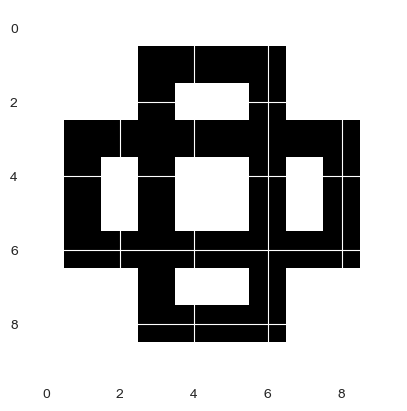
\includegraphics[width=\linewidth]{Figures/1st_geo.png}
%     \end{subfigure}
%     \hfill
%     \begin{subfigure}[b]{0.49\linewidth}
%         \centering
%         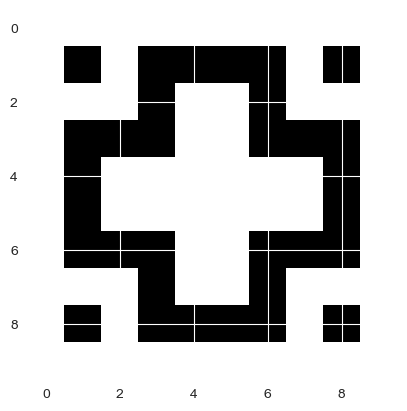
\includegraphics[width=\linewidth]{Figures/2nd_geo.png}
%     \end{subfigure}
%     \caption{The two design geometries used in the following studies.}
%     \label{fig:design_geos}    
% \end{figure}

\begin{figure}[h]
    \centering
    \begin{subfigure}{0.3\textwidth}
        \centering
        
\includegraphics[width=\textwidth]{FinalFigures/1st_geo.pdf}
        \vspace{-1cm}
        % \caption{}
        \label{fig:subfig-a}
    \end{subfigure}
    \hspace{-0.5cm}
    \begin{subfigure}{0.3\textwidth}
        \centering
        
\includegraphics[width=\textwidth]{FinalFigures/2nd_geo.pdf}
        \vspace{-1cm}
        % \caption{}
        \label{fig:subfig-b}
    \end{subfigure}
    \caption{Arbitrarily selected unit cell geometries for this paper's studies.}
    \label{fig:design_geos}
\end{figure}

\subsubsection{Dispersion Relations and Bandgaps}
\label{subsubsection:Dispersion Relations and Bandgaps}
Given the material properties and geometry of an acoustic metamaterial, its dispersion relation can be calculated by solving the Navier equations \citep[see][]{zhang2021realization},  
\begin{equation}
    (\lambda (\mathbf{r})+ \mu (\mathbf{r})) \nabla(\nabla \cdot \mathbf{u}) + \mu (\mathbf{r}) \nabla^2 \mathbf{u} = \rho (\mathbf{r}) \frac{\partial^2 \mathbf{u}}{\partial t^2} \label{eq1}
\end{equation} 
where $\lambda$ is the Lamé constant, $\mu$ is the shear modulus, $\mathbf{u}$ is the displacement vector, and $\rho$ is the density. 
Because regular metamaterials are formed by tiling a unit cell, we can reduce the domain of our analysis in Eq. \eqref{eq1} to a unit cell under Bloch-Floquet periodic boundary conditions. According to Bloch-Floquet theory, in a periodic domain, we can express the displacement field as \citep{yang2016effective}
\begin{equation}
    \mathbf{u}(\mathbf{r}+\mathbf{a}) = \mathbf{u}(\mathbf{r})e^{i\mathbf{k} \cdot \mathbf{a}}  \label{eq2}
\end{equation}
where $\mathbf{r}$ is the position vector, $\mathbf{a}$ is the lattice vector, and $\mathbf{k}$ is the wave vector. To solve Eq. \eqref{eq1} in our reduced domain, we discretize a unit cell using the finite element (FE) method and rewrite the formulation as a generalized eigenvalue problem.
\begin{equation}
    (\mathbf{K}(\mathbf{k}) - \omega^2 \mathbf{M})\mathbf{U} = \mathbf{0}  \label{eq3}
\end{equation}
where $\mathbf{K}$ and $\mathbf{M}$ are the stiffness and mass matrices of the unit cell respectively. By solving Eq. \eqref{eq3} with a finite element solver \rev{using flexible mesh sizes ranging from 10$\times$10 to 40$\times$40 pixel elements}, we can find the relation between eigenfrequency ($\omega$) and wave vector ($\mathbf{k}$), which forms the dispersion curves. By examining the dispersion curves, we can identify bandgaps where propagation of waves with certain frequencies is prohibited by the metamaterial \cite{bilal2011ultrawide}. \rev{Previous studies have shown that these FE computed bandgaps are experimentally verifiable, with discrepancies attributed partly to manufacturing inaccuracies. \cite{mazzotti2023bio, Bastawrous2024}} These bandgaps will be characterized in the following studies by their center frequency and bandwidth.

%%%%%%%%%%%%%%%%%%%%%%%%%%%%%%%%%%%%%%%%%%%%%%%%%%%%%%%%%%%%%%%%%%%%%%%%%%%%%%%%%%%%%%%%%%%%%%%%%%%%%%%%%%%%%%%%%%%%%
\subsection{Uncertainty Quantification}
\label{subsec:Uncertainty Quantification}
The purpose of UQ is to endow predictions with some probabilistic measure of confidence \citep{ghanem2017handbook}. One important aspect in UQ concerns the propagation of uncertainties (given some input-output model $f$) from the stochastic input space to an output quantity of interest. 
% , given some model and stochastic input space to that model, predict how the input stochasticity will propagate to the output space. In other words, UQ aims to map an input probability density to an output probability density. 
Let $\mathbf{X} = (X_1, X_2, \dots, X_m)^T$ represent our stochastic $m$-dimensional input to $f$ (with statistically independent components), defined on a probability space $(\Theta, \mathcal{F}, P)$. We denote by $P_{\mathbf{X}}$ the probability measure of $\mathbf{X}$, defined by the probability density function $p_{\mathbf{X}}$ with respect to the Lebesgue measure $d\mathbf{x}$ in $\mathbb{R}^m$: $P_{\mathbf{X}}(d\mathbf{x}) = p_{\mathbf{X}}(\mathbf{x})d\mathbf{x}$. Let $P_{\mathbf{Y}}$ be the pushed-forward (i.e., image) measure through $f$, associated with the stochastic $q$-dimensional output $\mathbf{Y} = f(\mathbf{X})$. We denote by $p_{\mathbf{Y}}$ the probability density function defining $P_{\mathbf{Y}}$.
% Suppose also that our model $f$ produces outputs $\mathbf{Y} = f(\mathbf{X})$ with an inherited probability density function $P(\mathbf{y})$ due to the stochasticity in $\mathbf{X}$. 
The task is then to estimate $P_{\mathbf{Y}}$, given $P_{\mathbf{X}}$. In the context of the metamaterials studies in this paper, $P_{\mathbf{X}}$ would be the probability measure of some material properties and geometric defects, whereas $P_{\mathbf{Y}}$ would be the probability measure of bandgap size and location. This can be achieved through various techniques, including Monte Carlo sampling and surrogate modeling methods. %In the studies that follow, we will demonstrate the utility of such approaches in capturing the stochasticity of acoustic metamaterial bandgap locations and sizes, given stochastic material properties, and geometric defects of the metamaterial unit cell.
%%%%%%%%%%%%%%%%%%%%%%%%%%%%%%%%%%%%%%%%%%%%%%%%%%%%%%%%%%%%%%%%%%%%%%%%%%%%%%%%%%%%%%%%%%%%%%%%%%%%%%%%%%%%%%%%%%%%%
\subsubsection{Monte Carlo Sampling}
The Monte Carlo (MC) approach involves the following steps:
\begin{enumerate}
    \item Generate a large number (M) of random samples $\mathbf{X}_1, \mathbf{X}_2, \dots, \mathbf{X}_M$, drawn from $P_{\mathbf{X}}$.
    \item Evaluate the associated output samples: $\mathbf{Y}_i = f(\mathbf{X}_i) \quad \text{for } i = 1,2, \dots, M$.
    \item Estimate $p_{\mathbf{Y}}$ (using a kernel density estimate, for instance) and/or analyze statistical moments of $\mathbf{Y}$ (e.g., the mean and the covariance matrix).
\end{enumerate}

Monte Carlo sampling approximates the true probability distribution with a large enough sample size but may be inefficient or infeasible in terms of computation cost to generate many samples of $\mathbf{X}$. This approach serves as a baseline that can be used to assess the relevance of alternative techniques, including the ones demonstrated in this paper.
%Whenever applicable (due to the computation associated with model evaluation for random instances of $\mathbf{X}$), this approach delivers baseline results that can be used to assess the relevance of alternative techniques, including the ones demonstrated in this paper.
%%%%%%%%%%%%%%%%%%%%%%%%%%%%%%%%%%%%%%%%%%%%%%%%%%%%%%%%%%%%%%%%%%%%%%%%%%%%%%%%%%%%%%%%%%%%%%%%%%%%%%%%%%%%%%%%%%%%%
\subsubsection{Polynomial Chaos Expansion (PCE)}
Polynomial Chaos Expansion (PCE) is used in this paper to construct computationally cheaper surrogate models to the assumed ground truth FE model. In this paper, PCE surrogate models are constructed by explicitly computing relatively few bandgap sizes and locations from material property and/or defective geometry samples. This surrogate model can then be sampled at negligible cost to reveal the statistical distribution of metamaterial bandgap properties given some stochasticity on material properties and geometry. This technique works by representing any given black-box model with smooth and bounded outputs as a linear combination of polynomial basis functions tailored to be orthogonal with respect to the input space probability distribution \cite{sudret2008global, crestaux2009polynomial}. This orthogonality property allows for each polynomial to capture unique information about the true black box model. A brief mathematical description of the method follows.

Assume that $\mathbf{Y} = f(\mathbf{X})$ is a second-order random variable, with $E\{\|\mathbf{Y}\|^2\} < + \infty$, where $E$ denotes the mathematical expectation and $\|\cdot\|$ is the standard Euclidean norm (in $\mathbb{R}^q$). The polynomial chaos expansion (PCE) of $\mathbf{Y}$ is then written as 
% Polynomial Chaos Expansion (PCE) is used in this paper to construct computationally cheaper surrogate models to the assumed ground truth, finite element analysis model. This technique can represent any given black-box model with smooth and bounded outputs as a linear combination of basis functions which are polynomials, to varying levels of accuracy depending on the degree of the polynomial basis functions permitted and the number of samples provided for fitting. The polynomials are crafted to be orthogonal with respect to the joint input probability density and this allows each of the basis polynomials to capture a different independent piece of information in some abstract sense about the relation between the input and output space, maximizing the information extracted from each sample.
% More rigorously, for some given random input vector \( \mathbf{X} \) and associated joint probability density function \( J(\mathbf{X}) \), PCE aims to express the uncertain output \( \mathbf{Y} \) as a function of \( \mathbf{X} \) in the form:
\begin{equation}
    \mathbf{Y} = \sum_{n=0}^{\infty} a_n \Phi_n(\mathbf{X})
\end{equation}
where $\{\Phi_n\}_{n \geq 0}$ are multivariate polynomials that are orthonormal with respect to $P_{\mathbf{X}}$ (that is, $E\{\Phi_n(\mathbf{X})\Phi_{n'}(\mathbf{X})\} = \delta_{nn'}$, where $\delta_{nn'}$ is the Kronecker delta), and $\{a_n\}_{n \geq 0}$ are expansion coefficients \citep{ghanem2003stochastic,ghanem2017handbook}. The above representation defines a surrogate model that, once calibrated, enables the characterization of $\mathbf{Y}$. The coefficients can be computed by exploiting the orthogonality of the Hilbertian basis:
\begin{equation}\label{eq:def-an}
    a_n = E\{f(\mathbf{X}) \Phi_n(\mathbf{X})\} = \int_{\mathbb{R}^m} f(\mathbf{x}) \Phi_n(\mathbf{x}) p_{\mathbf{X}}(\mathbf{x}) d\mathbf{x}
\end{equation}
% \[a_n = \frac{\int f(\mathbf{X}) \Phi_n(\mathbf{X}) J(\mathbf{X}) d\mathbf{X}}{\int \Phi_n^2(\mathbf{X}) J(\mathbf{X}) d\mathbf{X}}\]
% With orthogonal in this context defined as: 
% \[\int_{\Omega} \Phi_i(\mathbf{x}) \Phi_j(\mathbf{x}) J(\mathbf{x}) d\mathbf{x} &= \delta_{ij} \]
% where \( \Omega = \{\mathbf{x} \in \mathbb{R}^m : J(\mathbf{x}) > 0\} \) is the support of the m-dimensional random vector \( \mathbf{X} \) and \( \delta_{ij} \) is the Kronecker delta function.
The choice of the polynomials depends on the distribution on $\mathbf{X}$ \citep{Xiu-2002,Soize-2004}; see \Cref{tab:dist_PCE}.
\begin{table}[H]
    \caption{Example standard distributions and their associated basis polynomials.}
    \centering
    \begin{tabular}{cc} 
        \toprule
        Distribution & Basis Polynomials \\
        \midrule        
        Gaussian & Hermite \\
        Uniform & Legendre \\
        Gamma & Laguerre \\
        Beta & Jacobi \\
        \bottomrule
    \end{tabular}
    \label{tab:dist_PCE}
\end{table}
For arbitrary distributions, families of polynomial bases can be constructed via ad hoc orthonormalization techniques \citep{Perrin2012}. One common technique, which is implemented in the Python package Chaospy \citep{FEINBERG201546} and used in this paper, is the Stieltjes procedure \citep{stieltjes1884quelques}.

In practice, the PCE representation is truncated by restricting the polynomial order. Adopting a simplified notation (in lieu of the standard notation based on multi-indices), we write 
% depends on the truncation of the infinite series, which in practice, is often truncated at some low order \( N \). This results in the finite sum below, which represents the surrogate models we create and compare in this paper.
%\begin{equation} \mathbf{Y} = f(\mathbf{X}) \approx \sum_{n=0}^{N} a_n \Phi_n(\mathbf{X}) \label{eq1} \end{equation}
\begin{equation}
    \mathbf{Y} \approx \sum_{n=0}^{N} a_n \Phi_n(\mathbf{X})
\end{equation}
The above equation defines is a mean-square convergent approximation, implying that a convergence analysis must be performed with respect to $N$.

In this work, PCE expansions are generated with the Python package Chaospy, which is a general purpose UQ toolkit \citep{FEINBERG201546}. Some strategies to compute the PCE coefficients are reviewed in the next \Cref{subsubsec:spectral projection}.
%%%%%%%%%%%%%%%%%%%%%%%%%%%%%%%%%%%%%%%%%%%%%%%%%%%%%%%%%%%%%%%%%%%%%%%%%%%%%%%%%%%%%%%%%%%%%%%%%%%%%%%%%%%%%%%%%%%%%
\subsubsection{Evaluation of the Chaos Coefficients}
\label{subsubsec:spectral projection}
There exist various techniques to compute the set of coefficients $\{a_n\}_{n \geq 0}$, including intrusive and non-intrusive techniques; see \citep{le2010spectral,ghanem2017handbook} for reviews. 
% UQ aims to approximate $P(\mathbf{y})$ through sampling and surrogate modeling methods. One of these UQ methods is spectral projection. This technique has broad applications to many domains of engineering and science and is particularly useful when the model $f$ is complex. The benefits of spectral projection as a UQ technique are that (1.) it is non-intrusive, requiring no knowledge of the internal workings of the model $f$, (2.) it can be very efficient in sampling, requiring orders of magnitude less samples compared to simpler methods like Monte Carlo sampling, and (3.) it is compatible with surrogate modeling methods like polynomial chaos expansion, allowing for a construction of substantially cheaper alternatives to computationally expensive and complex (for example finite element analysis) models. 
% spectral projection is a method for strategically selecting points \( \mathbf{X}_i \) in the input space to evaluate the model \( f \) at to maximize, in some abstract sense, the information gained about the model and output space per sample. 
In this paper, we consider the following techniques to generate sample nodes to compute the chaos coefficients according to spectral projection Eq.~\eqref{eq:def-an} (and rely on their implementation in the Python package Chaospy) \rev{These techniques are standard in the field of UQ and more details on their mathematical description and advantages/disadvantages can be found in the UQ handbook. \cite{ghanem2017handbook}}.
\begin{itemize}
    \item \textbf{Monte Carlo sampling}: in this case, the mathematical expectation in Eq.~\eqref{eq:def-an} is estimated through 
    \begin{equation}
        a_n \approx \frac{1}{M} \sum_{i = 1}^M f(\mathbf{X}_i) \Phi_n(\mathbf{X}_i)
    \end{equation}
    This strategy presents a low convergence rate (note that this drawback can be partially circumvented using more efficient sampling strategies), which is however independent of $m$ (the dimension of the stochastic input). It remains applicable when the forward model $f$ is reasonably cheap to evaluate. 
    
    % In this sampling strategy, points \( \mathbf{X}_i \) are drawn randomly according to the probability density function \( J(\mathbf{X}) \) but instead of inferring \( P(\mathbf{Y}) \) from the input and output pairs, the pairs are fitted to the PCE surrogate model which can then be sampled relatively cheaply and with high fidelity to the true model \( f \)  to recover an approximate output probability density function \( P_{PCE}(\mathbf{Y}) \).

    \item \textbf{Quadrature rule}:
    Alternatively, the integral in Eq.~\eqref{eq:def-an} can be evaluated using a deterministic (e.g., Gaussian) quadrature rule:
    \begin{equation}
        a_n \approx \sum_{i=1}^{N_Q} w_i f(\mathbf{X}_i)
    \end{equation}
    where $\{w_i\}_{i = 1}^{N_Q}$ and $\{\mathbf{X}_i\}_{i = 1}^{N_Q}$ denote the weights and nodes of the $N_Q$-point cubature. Such rules are typically formulated using a tensorization of one-dimensional cubatures when $m >1$. \rev{Notably, this method suffers from the curse of dimensionality, requiring a sample number $N_Q=(N_{PD}-1)^m$, where $N_{PD}$ is the PCE degree.}   
    % In quadrature rule sampling, input points ("nodes") \( \mathbf{X}_i \) are selected at the roots of the orthogonal PCE polynomials \( \Phi_n(\mathbf{X}) \). 
    % These nodes are also assigned a weight \( w_i \) which are also derived from \( \Phi_n(\mathbf{X}) \) (with different formulae for different basis sets due to normalization requirements) and signify to the relative influence of each node on the expected value of \(f(\mathbf{X})\). 
    % \[
    % \int f(\mathbf{X}) J(\mathbf{X}) d\mathbf{X} \approx \sum_{i=1}^{N} w_i f(\mathbf{X}_i)
    % \]
    % These nodes, weights, and their evaluations using the model \(f\) are then used to fit the PCE surrogate model, from which we can extract approximations of the true output space probability density \( P_{PCE}(\mathbf{Y}) \). Because the nodes are polynomial roots and weights and nodes are paired, this implies that the number of quadrature nodes and weights are both a function of the truncation order \( N \) of the PCE polynomial basis. Specifically, the number of nodes/weights generated is \((N+1)^m\), an exponential relationship that is often referred to as the "curse of dimensionality". This \( N \) from here onwards will be referred to as the degree of the quadrature.
    
    \item \textbf{Smolyak sparse grid}:
    In order to circumvent the curse of dimensionality arising in tensor product formula, a sparse grid can be used where a subset of quadrature points is identified based on a given criterion (constraining the sum of all one-dimensional levels of accuracy). This leads to a much smaller number of quadrature points, and enables integration for large values of $m$. Here we use the Smolyak sparse grid introduced in \citep{Smolyak}.
    % The quadrature rule sampling strategy above can be thought of as sampling roots to a full tensor product of 1D polynomials \( \Phi_n(X_1), \Phi_n(X_2) ... \Phi_n(X_m) \) for the m-dimensional input space. This effectively is sampling over a grid of points in m-dimensional space. The sparse grid approach refines this sampling strategy by combining quadrature grid points of different resolutions up to some order N while discarding others to form a subset of the full tensor grid with the number of points scaling as \( N \cdot (\log N)^{m-1} \) which is considerably more impervious to the exponential scaling problem than the quadrature rule sampling strategy.
\end{itemize}

%%%%%%%%%%%%%%%%%%%%%%%%%%%%%%%%%%%%%%%%%%%%%%%%%%%%%%%%%%%%%%%%%%%%%%%%%%%%%%%%%%%%%%%%%%%%%%%%%%%%%%%%%%%%%%%%%%%%%
\subsubsection{Geometry Defects}
\label{subsubsec:m_geo}

As seen in \Cref{subsubsec:spectral projection}, the dimensionality of the input space severely affects the amount of computation needed to generate PCE surrogate models. Thus, there is intrinsic motivation to keep input space dimensionality low, leading to the natural issue of dealing with increasing resolution and the quadratic scaling in pixel count for 2D metamaterials. It would be infeasible in practice to use a method which requires one dimension input for every pixel in a geometry, and such a method would only work for very crude geometry representations. 

In manufacturing processes, the stochastic nature of defects is not usually a function of the arbitrary resolution one chooses to represent their geometry with, but instead of some scale independent parameter such as lithography laser precision, 3D printing nozzle size, or mill head diameter in CNC machining. Motivated by this, we sought a single scale invariant parameter which define stochastic defects on the designed geometry, and decided to use an edge pixel ``flip proportion'' (FP) parameter. Our algorithm for generating geometry defects with this FP parameter is as follows. 
\begin{enumerate}
    \item Design a defect-free geometry. 
    \item Identify all the edge pixels in the design geometry. These are stiff material pixels which share an edge with a soft material pixel, or vice versa.
    \item Randomly pick a proportion of the edge pixels equal to FP and flip these pixels to the other material.
\end{enumerate}

% \begin{figure}[H]
%     \centering
%     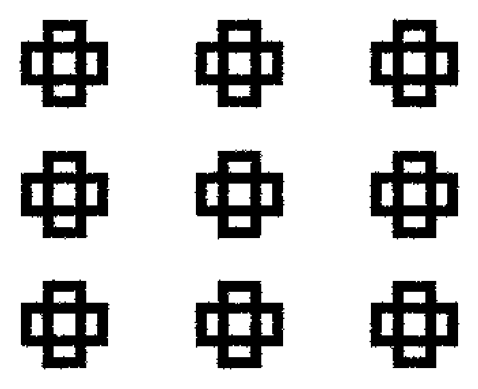
\includegraphics[width=0.75\linewidth]{Figures/defect_palette_40.png}
%     \caption{A palette of possible defective shapes for the same FP parameter of 0.05 (5\% flip rate)}
%     \label{fig:defect_palette_40}
% \end{figure}

\begin{figure}[H]
    \centering
    \begin{subfigure}{0.25\textwidth}
        \centering
        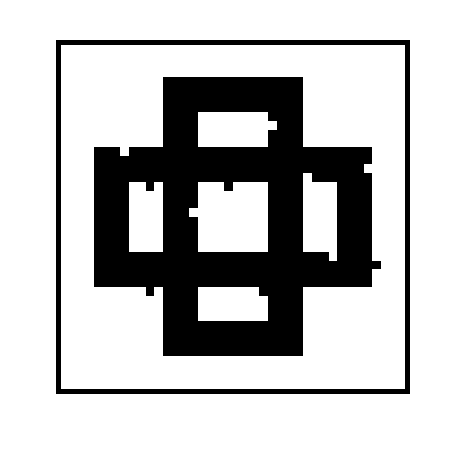
\includegraphics[width=\textwidth]{FinalFigures/defect_palette_40_a.pdf}
        \vspace{-1.4cm}
        % \caption{}
        \label{fig:subfig-1}
    \end{subfigure}
    \hspace{-0.6cm}
    \begin{subfigure}{0.25\textwidth}
        \centering
        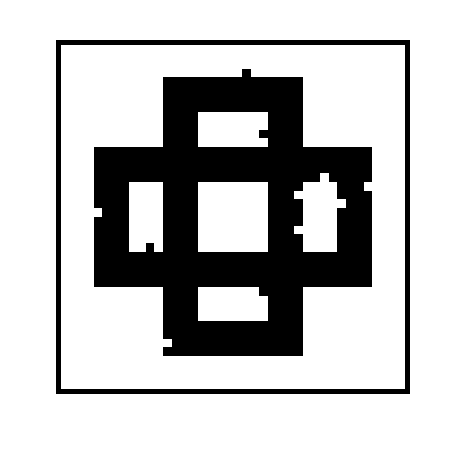
\includegraphics[width=\textwidth]{FinalFigures/defect_palette_40_b.pdf}
        \vspace{-1.4cm}
        % \caption{}
        \label{fig:subfig-2}
    \end{subfigure}
    \hspace{-0.6cm}
    \begin{subfigure}{0.25\textwidth}
        \centering
        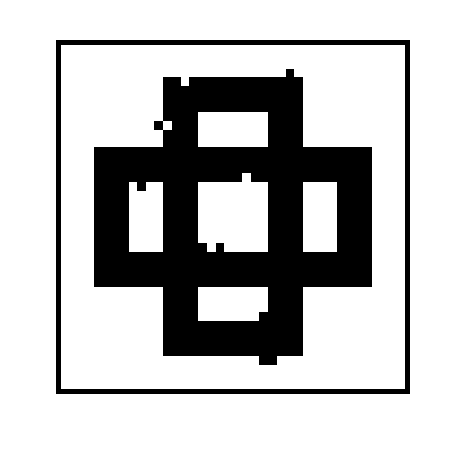
\includegraphics[width=\textwidth]{FinalFigures/defect_palette_40_c.pdf}
        \vspace{-1.4cm}
        % \caption{}
        \label{fig:subfig-3}
    \end{subfigure}
    \hspace{-0.6cm}
    \vspace{0.1cm}
    
    \begin{subfigure}{0.25\textwidth}
        \centering
        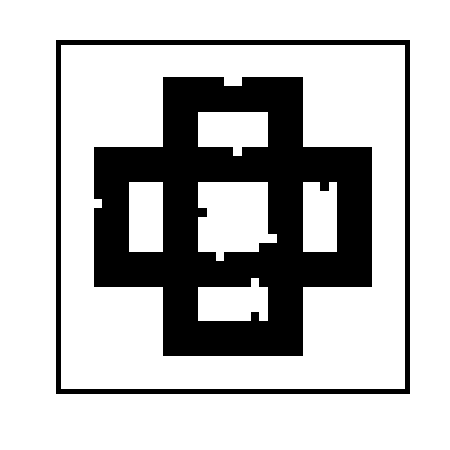
\includegraphics[width=\textwidth]{FinalFigures/defect_palette_40_d.pdf}
        \vspace{-1.4cm}
        % \caption{}
        \label{fig:subfig-4}
    \end{subfigure}
    \hspace{-0.6cm}
    \begin{subfigure}{0.25\textwidth}
        \centering
        
\includegraphics[width=\textwidth]{FinalFigures/defect_palette_40_e.pdf}
        \vspace{-1.4cm}
        % \caption{}
        \label{fig:subfig-5}
    \end{subfigure}
    \hspace{-0.6cm}
    \begin{subfigure}{0.25\textwidth}
        \centering
        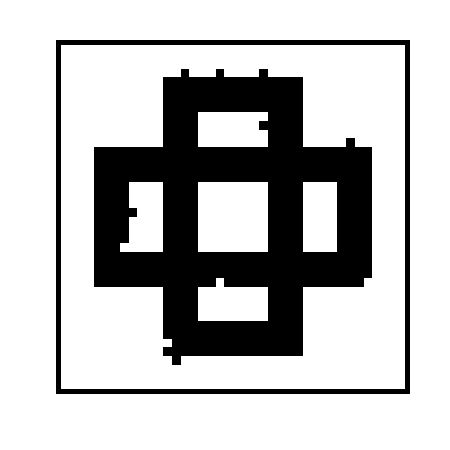
\includegraphics[width=\textwidth]{FinalFigures/defect_palette_40_f.pdf}
        \vspace{-1.4cm}
        % \caption{}
        \label{fig:subfig-6}
    \end{subfigure}
    \hspace{-0.6cm}
    \vspace{0.1cm}
    
    \begin{subfigure}{0.25\textwidth}
        \centering
        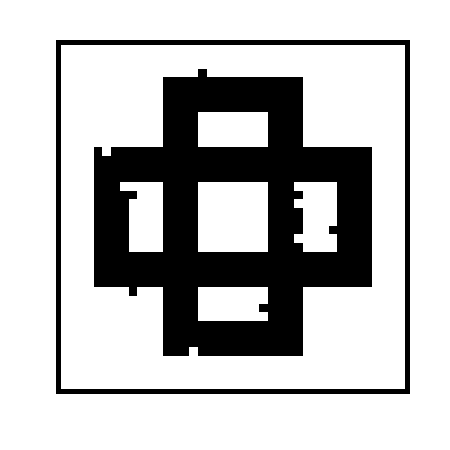
\includegraphics[width=\textwidth]{FinalFigures/defect_palette_40_g.pdf}
        \vspace{-1.4cm}
        % \caption{}
        \label{fig:subfig-7}
    \end{subfigure}
    \hspace{-0.6cm}
    \begin{subfigure}{0.25\textwidth}
        \centering
        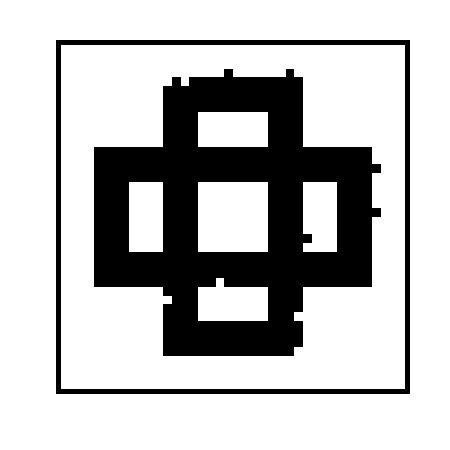
\includegraphics[width=\textwidth]{FinalFigures/defect_palette_40_h.pdf}
        \vspace{-1.4cm}
        % \caption{}
        \label{fig:subfig-8}
    \end{subfigure}
    \hspace{-0.6cm}
    \begin{subfigure}{0.25\textwidth}
        \centering
        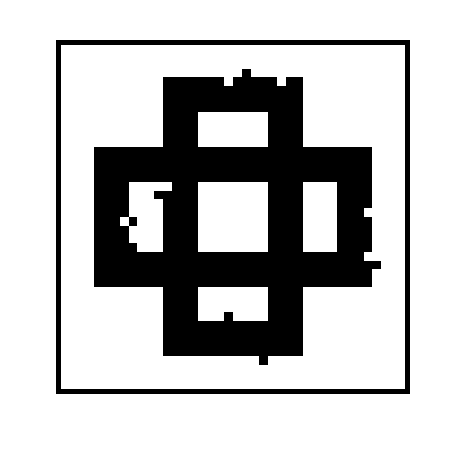
\includegraphics[width=\textwidth]{FinalFigures/defect_palette_40_i.pdf}
        \vspace{-1.4cm}
        % \caption{}
        \label{fig:subfig-9}
    \end{subfigure}
    \hspace{-0.5cm}
    \caption{Palette of possible defective geometries for the same flip proportion parameter ($FP = 5 \%$).}
    \label{fig:defect_palette_40}
\end{figure}

The main benefit of this algorithm is that it offers a way to capture realistic cases of processing defects with a single scale invariant parameter. 

There are three concerns with this algorithm. The first is that only edge pixels can be flipped. Because the most serious defects and deviations in manufacturing occur at the edges of geometries, we chose to limit the flipping to only edge pixels. However, our algorithm is capable of flipping a proportion of all pixels. 

The second concern is that this algorithm no longer leads to a deterministic output space as multiple defective geometries are possible for the same FP \ref{fig:defect_palette_40}. This leads to the question of whether the FP parameter is a valid representation of the input geometry. If the possible model outputs from a single FP parameter, all else held fixed, varies wildly, then this would cause problems with the PCE fitting process as the fit cannot satisfy multivalued functions. If instead the output variation due to from a FP  is small relative to the average variation caused by different FP values, then this FP method is a pseudo-deterministic scenario where the variation introduced by multivalued defective geometries can be considered model noise in an otherwise deterministic model and PCE will have a good chance of successfully fitting surrogate models. This variation comparison will be tested in results presented in \Cref{subsec:r_geo}. 

A third concern is that because only edge pixels are flipped, as resolution increases, less of the shape area is comprised of edge pixels and thus less area is subject to random flipping. This problem was examined by looking for convergence in the effects of defects as the shape resolution increased, with results also presented in \Cref{subsec:r_geo}. 
%%%%%%%%%%%%%%%%%%%%%%%%%%%%%%%%%%%%%%%%%%%%%%%%%%%%%%%%%%%%%%%%%%%%%%%%%%%%%%%%%%%%%%%%%%%%%%%%%%%%%%%%%%%%%%%%%%%%%
\section{Results and Discussion}
\label{sec:Results}
The following subsections detail the accuracy of the UQ techniques (see \Cref{subsec:Uncertainty Quantification}) in representing the true statistical distribution of bandgap sizes and locations given  in 1D (material property) and 7D (material properties and geometric defects) stochastic input space scenarios. The techniques will be demonstrated in the following sections on 4 different types of standard distributions, the uniform, normal, gamma, and beta, and for two different design geometries. For purposes of brevity, not all combinations of distributions and methods are shown in the following results, but the methods do generalize to all distributions examined in this paper. 
%\label{}
%\subsection{1D Uniform Input Space}
%%%%%%%%%%%%%%%%%%%%%%%%%%%%%%%%%%%%%%%%%%%%%%%%%%%%%%%%%%%%%%%%%%%%%%%%%%%%%%%%%%%%%%%%%%%%%%%%%%%%%%%%%%%%%%%%%%%%%
\subsection{Geometry Resolution Effects on Bandgap Computations}
\label{subsec:r_geo}
In this study, we examine the effects of increasing geometry resolution on the FE solver outputs, and investigate whether the FP parameter is a viable scale invariant way to represent geometric defects. In general, for FE solvers, the more crude the resolution, and the fewer the elements, the more error there will be in the FE calculations. Mesh refinement techniques are typically used to strategically refine the resolution at places where more accuracy is needed or where rapid transitions in geometry or loadings occur. For our 2D unit cell design, we scale geometry resolution from 10$\times$10 to 100$\times$100 pixels and plot the FE solver outputs in \Cref{fig:FEM_convergence_afo_resolution}.

% \begin{figure}[H]
% 	\centering 
% 	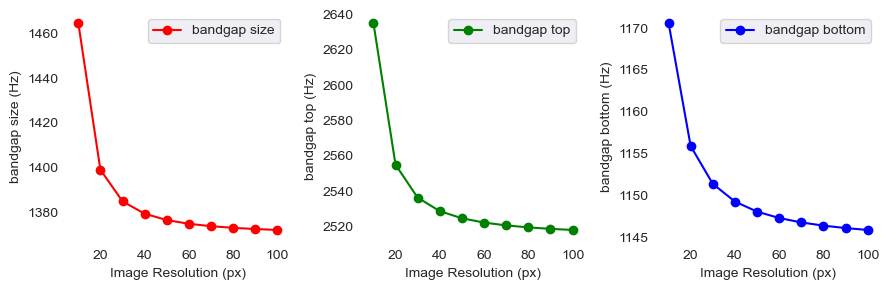
\includegraphics[width=\textwidth]{Figures/P_FEM_convergence_afo_resolution.png}	
% 	\caption{The bandgap size, top, and bottom locations of a random sample defect geometry scaled by 1$\times$ to 10$\times$ in length, as computed by the finite element solver. Note in this case, the flipping of pixels were applied before resolution scaling.} 
% 	\label{fig:FEM_convergence_afo_resolution}%
% \end{figure}

\begin{figure}[H]
    \centering
    \begin{subfigure}{0.4\textwidth}
        \centering
        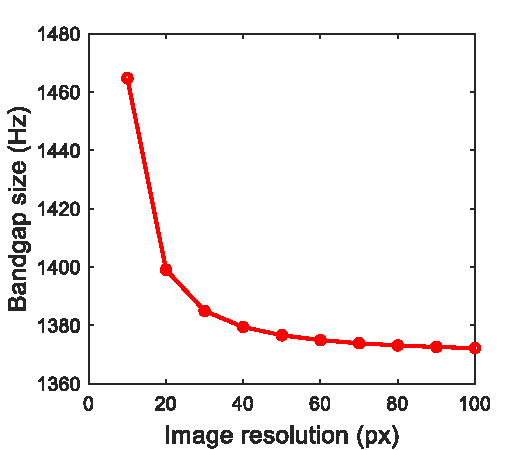
\includegraphics[width=\textwidth]{FinalFigures/P_FEM_convergence_afo_resolution_a.pdf}
        \caption{}
        \label{fig:subfig-1}
    \end{subfigure}\quad
    \begin{subfigure}{0.4\textwidth}
        \centering
        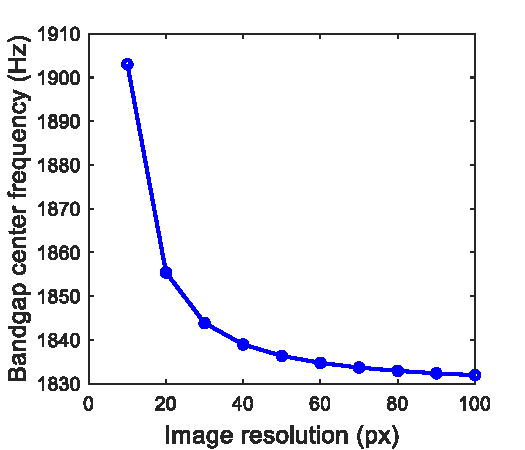
\includegraphics[width=\textwidth]{FinalFigures/P_FEM_convergence_afo_resolution_b.pdf}
        \caption{}
        \label{fig:subfig-2}
    \end{subfigure}    
    \caption{The bandgap size a) and center location b) of a random but representative sample defect geometry scaled in resolution by 1$\times$ to 10$\times$ in length (10 pixels to 100 pixels edge length), as computed by the finite element solver. The flipping of pixels was applied before resolution scaling. From this figure we gather that 40$\times$40 pixel resolution yields sufficiently good accuracy relative to the sizes of bandgap perturbations introduced by stochastic input parameters.}
    \label{fig:FEM_convergence_afo_resolution}
\end{figure}

% \begin{figure}[H]
% 	\centering 
% 	\includegraphics[width=0.8\textwidth]{FinalFigures/Fig3.pdf}	
% 	\caption{The bandgap size, top, and bottom locations of a random sample defect geometry scaled by 1$\times$ to 10$\times$ in length, as computed by the finite element solver. Note in this case, the flipping of pixels were applied before resolution scaling.} 
% 	\label{fig:FEM_convergence_afo_resolution}%
% \end{figure}

\Cref{fig:FEM_convergence_afo_resolution} shows a clear asymptotic trend of output values as resolution increases. For low image resolutions of 10 to 30 pixels, substantially higher error is introduced into the finite element model from elements being too crude in resolution. As the resolution increases to 40 pixels and above, there are diminishing returns on approximating the asymptotic output value and quadratically increasing computational effort. At 40$\times$40 pixels, the error is less than 1\% ($\sim 10^0\,\text{Hz}$) of the asymptotic value, and this error is about two orders of magnitude smaller than the effects of varying other parameters. Therefore, for the rest of the studies in this paper, geometries were generated and computed with a resolution of 40$\times$40 pixels. \rev{The FEA mesh used for each sample computation is also the same as the pixel geometry, because the same figure above suggests that beyond a 40$\times$40 pixel mesh, the predictions of the quantities of interest have converged}.

With FE solver convergence confirmed, we next investigate the concern regarding the ``flip proportion'' (FP) defect generation parameter. Since our algorithm only flips edge pixels, a higher image resolution implies a smaller proportion of the total pixels that are subject to flipping. As a result, flipping at higher resolution likely has smaller effects on bandgap outputs. To check how bandgap size and location distributions changes with increasing resolution, we hold FP constant and vary the geometry resolution from 10$\times$10 to 70$\times$70 pixels, computing the bandgap size, top, and bottom. Note that because our algorithm is pseudo-deterministic, with one FP parameter yielding multiple similar but different possible defect geometries, we average over 100 samples to obtain a statistically significant representation of effects from possible defect geometries from the same FP parameter. The results are shown in \Cref{fig:geo_defect_fp_convergence}.

% \begin{figure}[H]
%     \centering
%     \begin{subfigure}[b]{0.49\linewidth}
%         \centering
%         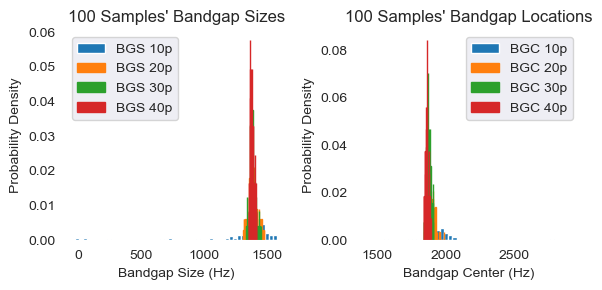
\includegraphics[width=\linewidth]{Figures/P_geo_defect_fp_convergence_10p-40p.png}
%         \caption{Histogram of computed bandgap size (left) and center location (right) of 100 geometry defect samples generated with the same FP value of 0.05 and paired with the same material properties for pixel resolutions of 10$\times$10, 20$\times$20, 30$\times$30, and 40$\times$40.}
%         \label{fig:geo_defect_fp_convergence_10p-40p}
%     \end{subfigure}
%     \hfill
%     \begin{subfigure}[b]{0.49\linewidth}
%         \centering
%         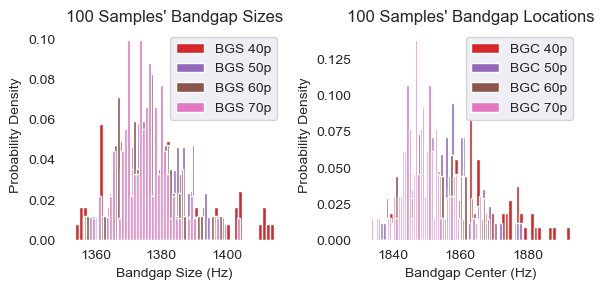
\includegraphics[width=\linewidth]{Figures/P_geo_defect_fp_convergence_40p-70p.png}
%         \caption{Histogram of computed bandgap size (left) and center location (right) of 100 geometry defect samples generated with the same FP value of 0.05 and paired with the same material properties for pixel resolutions of 40$\times$40, 50$\times$50, 60$\times$60, and 70$\times$70.}
%         \label{fig:geo_defect_fp_convergence_40p-70p}
%     \end{subfigure}
%     \caption{Results of study on variation introduced by non-deterministic FP parameter in generating geometric defects.}
%     \label{fig:geo_defect_fp_convergence}    
% \end{figure}

\begin{figure}[H]
    \centering
    \begin{subfigure}{0.45\textwidth}
        \centering
        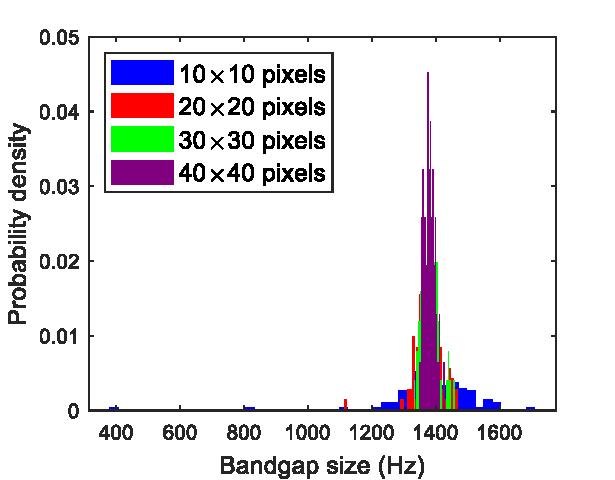
\includegraphics[width=\textwidth]{FinalFigures/P_geo_defect_fp_convergence_40p-70p_a.pdf}
        \caption{}
        \label{fig:subfig-1}
    \end{subfigure}\quad 
    \begin{subfigure}{0.45\textwidth}
        \centering
        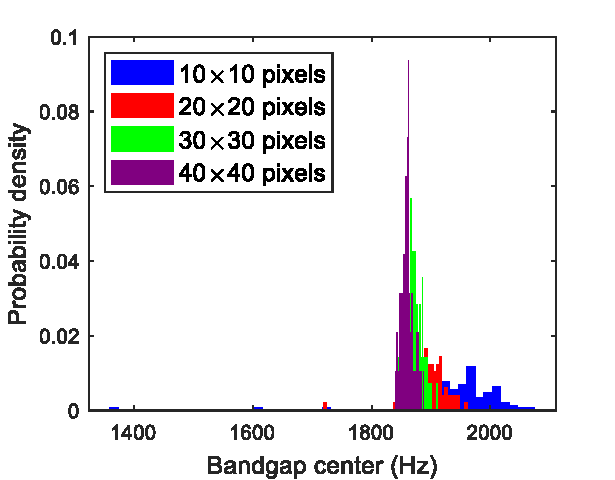
\includegraphics[width=\textwidth]{FinalFigures/P_geo_defect_fp_convergence_40p-70p_b.pdf}
        \caption{}
        \label{fig:subfig-2}
    \end{subfigure}
    
    \vspace{0.1cm}
    
    \begin{subfigure}{0.45\textwidth}
        \centering
        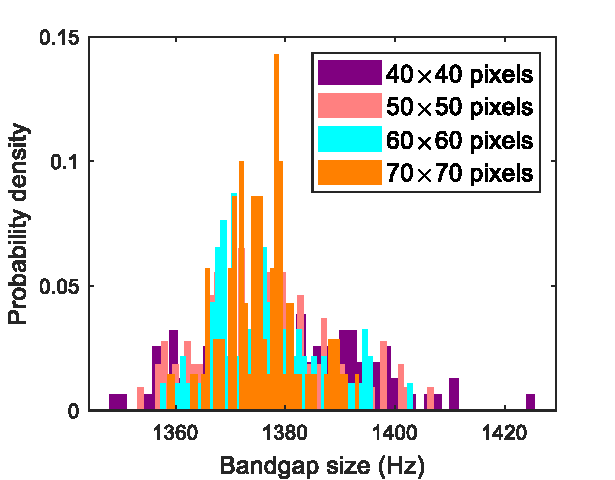
\includegraphics[width=\textwidth]{FinalFigures/P_geo_defect_fp_convergence_40p-70p_c.pdf}
        \caption{}
        \label{fig:subfig-3}
    \end{subfigure}\quad % Remove the space between subfigures
    \begin{subfigure}{0.45\textwidth}
        \centering
        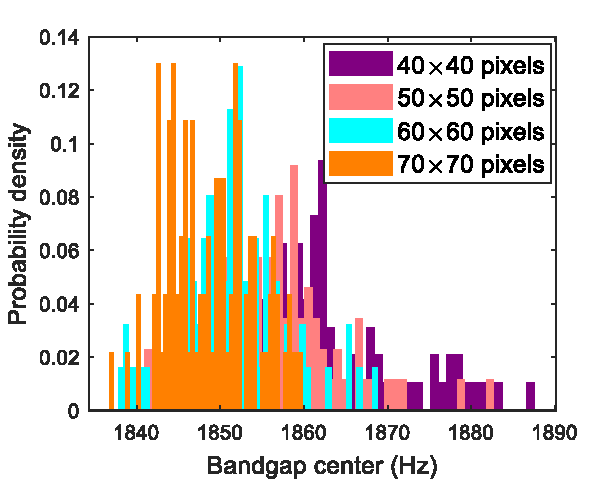
\includegraphics[width=\textwidth]{FinalFigures/P_geo_defect_fp_convergence_40p-70p_d.pdf}
        \caption{}
        \label{fig:subfig-4}
    \end{subfigure}
    
    \caption{Study results on output variation introduced by non-deterministic FP parameter for generating geometric defects. Histogram of computed a) bandgap size and b) center frequency of 100 geometrically defective samples generated with the same FP value of 0.05 and paired with the same material properties for pixel resolutions of 10$\times$10, 20$\times$20, 30$\times$30, and 40$\times$40. Histogram of computed bandgap c) size and d) center frequency location of 100 geometrically defective samples generated with the same FP value of 0.05 and paired with the same material properties for pixel resolutions of 40$\times$40, 50$\times$50, 60$\times$60, and 70$\times$70. Resolutions at 40$\times$40 and above can be considered to be convergent relative to the bandgap variations introduced by material property stochasticity.}
    \label{fig:geo_defect_fp_convergence}
\end{figure}

From FE computations on realistic stochastic material property ranges, it was found that output ranges for bandgap size and center position spanned several hundred Hertz. Therefore we would want any noise effects like the differences between defect geometries of the same FP to be well below this magnitude in variation. \Cref{fig:geo_defect_fp_convergence} shows that at below 30 pixels, we have unacceptably large variations in the hundreds to even thousands of Hz, due to each flipped pixel removing or adding a relatively large portion of the overall structure. At over 40 pixel image resolution, the variance from the many possible defective geometries starts to be convergent asymptotically to a range on the order of tens of Hertz. This means that the variation within a single FP value (noise) is at least an order of magnitude lower relative to the variation introduced by the stochastic material properties and FP value (signal). This result suggests that FP can be considered to be effectively deterministic and used as a valid representation of geometric defects. Furthermore, because the defect rate is primarily the deterministic parameter of bandgap properties, and not the specific pixel locations of defects, our assumption of periodic tiling in the defective geometry case is also validated, which makes for simpler computation. Thus for following studies, each set of sampled material properties will be paired with one defective geometry randomly generated with a sampled FP parameter.
%%%%%%%%%%%%%%%%%%%%%%%%%%%%%%%%%%%%%%%%%%%%%%%%%%%%%%%%%%%%%%%%%%%%%%%%%%%%%%%%%%%%%%%%%%%%%%%%%%%%%%%%%%%%%%%%%%%%%
\subsection{6D Gamma + 1D Beta (Material Properties + Geometry) Input Study}
\label{subsec:7D Gamma Input Space}

In this study, the stochastic (independent) input parameters include six material properties, assumed to be gamma distributed, and the geometry defect parameter FP, assumed to be beta distributed. The definition of the material property distributions follows the previous works \citep{Guilleminot_Soize_2013,Staber2017} which showed, using information theory, that the gamma distribution constitutes an objective choice in stochastic isotropic elasticity. The choice of beta distribution ensures that the geometry flip proportion parameter takes values between 0 and 1. The distribution parameters are provided in \Cref{7D_Gamma_Input_Table}, and the associated histograms for Monte Carlo sampling are shown in \Cref{fig:7d_gamma_input_mc_10000}: 

\begin{table}[H]
\centering
%\small
\tiny
\caption{7D Gamma Material Property \& Beta Geometry Input Distributions}
\label{7D_Gamma_Input_Table}
\begin{tabularx}{\linewidth}{Xccccc} 
\toprule
Material Property & Distribution & Mean ($\mu$) & Standard Deviation ($\sigma$) & Shape ($\alpha$) & Rate/Shape ($\beta$) \\
\midrule
\( \text{Soft bulk modulus } (K_{soft})\) & \( \text{Gamma} \) & \( 278 \text{ MPa} \) & \( 0.08\mu \) & \( 1.56\cdot10^2 \) & \( 1.78\cdot10^6 \) \\
\( \text{Stiff bulk modulus } (K_{stiff})\) & \( \text{Gamma} \) & \( 152 \text{ GPa} \) & \( 0.02\mu \) & \( 2.50\cdot10^3 \) & \( 6.06\cdot10^7 \) \\
\( \text{Soft shear modulus } (G_{soft})\) & \( \text{Gamma} \) & \( 72.5 \text{ MPa} \) & \( 0.08\mu \) & \( 1.56\cdot10^2 \) & \( 4.64\cdot10^5 \) \\
\( \text{Stiff shear modulus } (G_{stiff})\) & \( \text{Gamma} \) & \( 78.1 \text{ GPa} \) & \( 0.02\mu \) & \( 2.50\cdot10^3 \) & \( 3.13\cdot10^7 \) \\
\( \text{Soft density } (\rho_{soft})\) & \( \text{Gamma} \) & \( 1000 \text{ kg/m$^3$} \) & \( 0.08\mu \) & \( 1.56\cdot10^2 \) & \( 6.4 \) \\
\( \text{Stiff density } (\rho_{stiff})\) & \( \text{Gamma} \) & \( 8000 \text{ kg/m$^3$} \) & \( 0.02\mu \) & \( 2.50\cdot10^3 \) & \( 3.2 \) \\
\( \text{Geometry flip proportion }  (FP)\) & \( \text{Beta} \) & \( 0.025 \) & \( 0.08\mu \) & \( 1.52\cdot10^2 \) & \( 5.94\cdot10^3 \) \\
\bottomrule
\end{tabularx}
\end{table}

% \begin{figure}[H]
% 	\centering 
% 	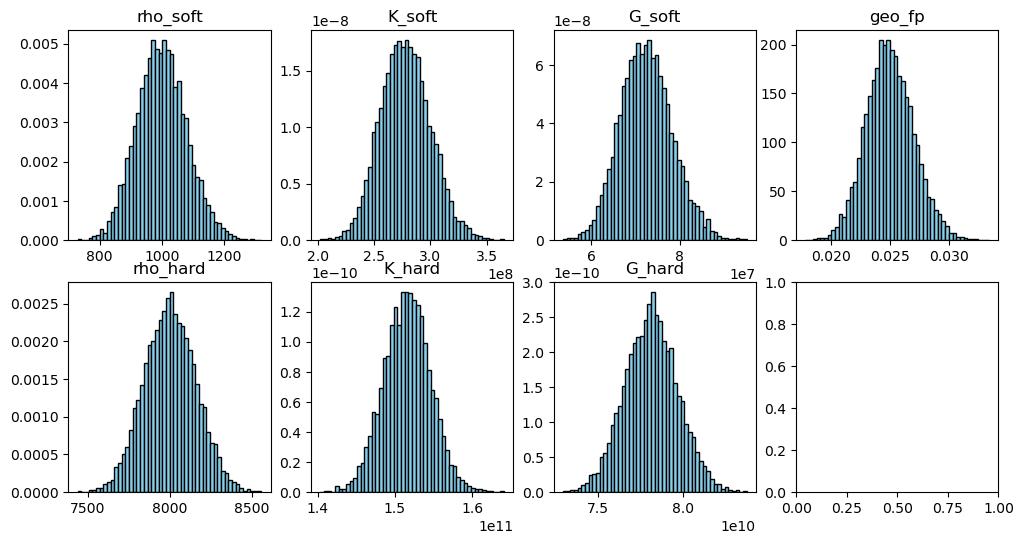
\includegraphics[width=\textwidth]{Figures/P_7d_gamma_input_mc_10000.png}	
% 	\caption{10000 Monte Carlo samples of the 7D Gamma and Beta input space, for visualization of the input space distribution shapes.} 
% 	\label{7d_gamma_input_mc_10000}%
% \end{figure}

\begin{figure}[H]
    \centering
    \begin{subfigure}{0.24\textwidth}
        \centering
        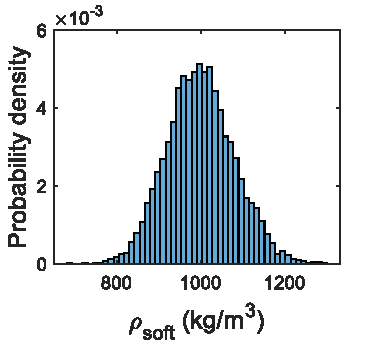
\includegraphics[width=\textwidth]{FinalFigures/P_7d_gamma_input_mc_10000_a.pdf}
        \caption{}
        \label{fig:subfig-1}
    \end{subfigure}
    \hspace{0.02\textwidth}
    \begin{subfigure}{0.24\textwidth}
        \centering
        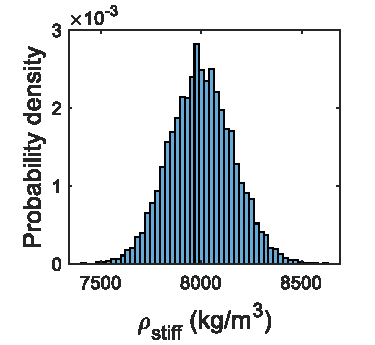
\includegraphics[width=\textwidth]{FinalFigures/P_7d_gamma_input_mc_10000_b.pdf}
        \caption{}
        \label{fig:subfig-2}
    \end{subfigure}
    \hspace{0.02\textwidth}
    \begin{subfigure}{0.24\textwidth}
        \centering
        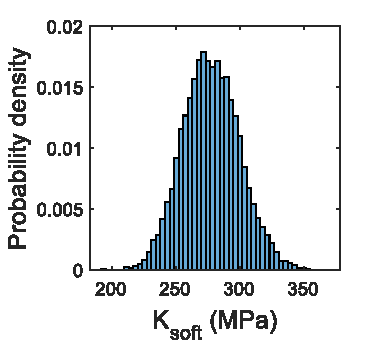
\includegraphics[width=\textwidth]{FinalFigures/P_7d_gamma_input_mc_10000_c.pdf}
        \caption{}
        \label{fig:subfig-3}
    \end{subfigure}
    
    \medskip
    
    \begin{subfigure}{0.24\textwidth}
        \centering
        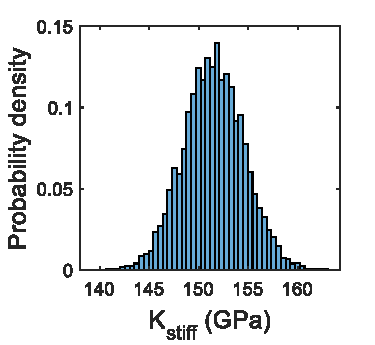
\includegraphics[width=\textwidth]{FinalFigures/P_7d_gamma_input_mc_10000_d.pdf}
        \caption{}
        \label{fig:subfig-4}
    \end{subfigure}
    \hfill
    \begin{subfigure}{0.24\textwidth}
        \centering
        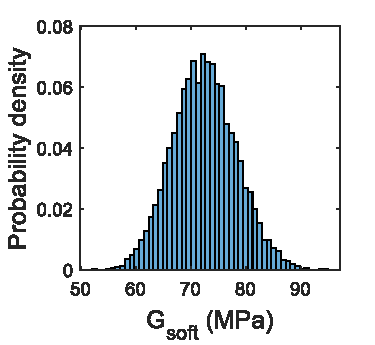
\includegraphics[width=\textwidth]{FinalFigures/P_7d_gamma_input_mc_10000_e.pdf}
        \caption{}
        \label{fig:subfig-5}
    \end{subfigure}
    \hfill
    \begin{subfigure}{0.24\textwidth}
        \centering
        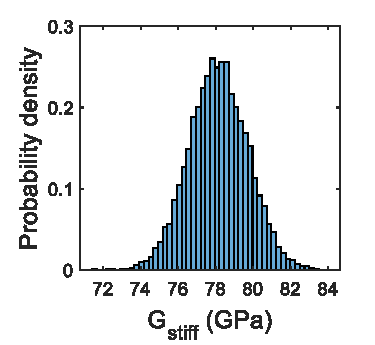
\includegraphics[width=\textwidth]{FinalFigures/P_7d_gamma_input_mc_10000_f.pdf}
        \caption{}
        \label{fig:subfig-6}
    \end{subfigure}
    \hfill
    \begin{subfigure}{0.24\textwidth}
        \centering
        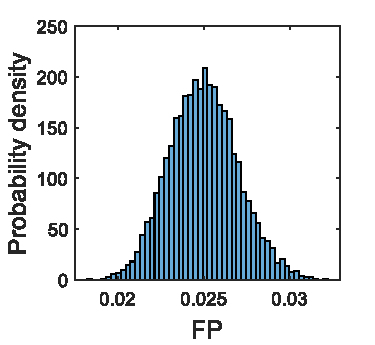
\includegraphics[width=\textwidth]{FinalFigures/P_7d_gamma_input_mc_10000_g.pdf}
        \caption{}
        \label{fig:subfig-7}
    \end{subfigure}
    
    \caption{10000 Monte Carlo samples of the 7D gamma and beta input space, for visualization of the input space distribution shapes, for a) density of the soft material, b) density of the stiff material, c) bulk modulus of the soft material, d) bulk modulus of the stiff material, e) shear modulus of the soft material, f) shear modulus of the stiff material, and g) the flip proportion parameter for generating geometry defects.}
    \label{fig:7d_gamma_input_mc_10000}
\end{figure}

The sampled geometry FP parameters are then used to randomly generate defective geometries to pair with each set of sampled material properties. The typical process and result of the geometry defect generation process is shown in \Cref{fig:defect_trio_1st_geo}.
% \begin{figure}[H]
% 	\centering 
% 	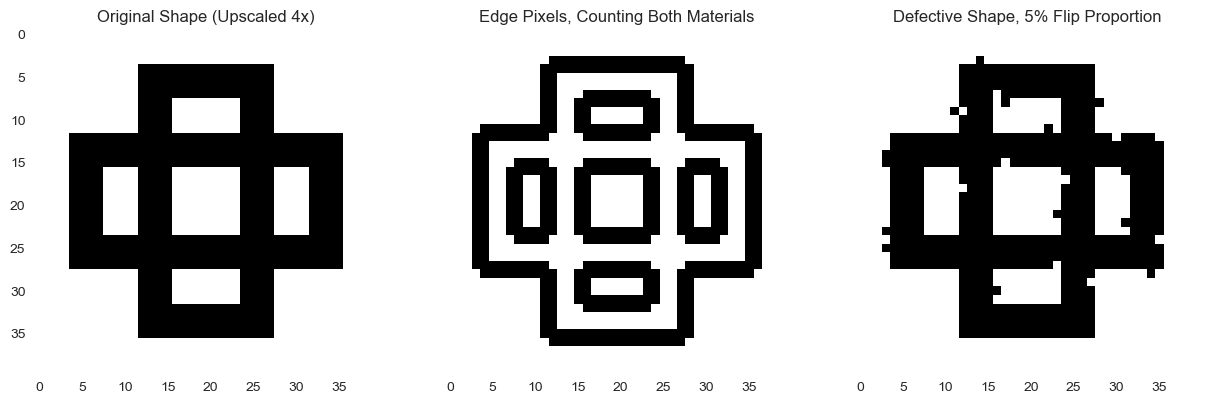
\includegraphics[width=\textwidth]{Figures/defect_trio_1st_geo.png}	
% 	\caption{Left: The defect free designed geometry, scaled up to 40px by 40px. Center: edge pixels of the design geometry, which will be subjected to random flipping at preset proportion of the FP parameter. Right: one resulting defective geometry after flipping edge pixels. This defect is a representative sample for illustration purposes. Different randomly generated defects are paired with each material property input.} 
% 	\label{defect_trio_1st_geo}%
% \end{figure}

\begin{figure}[H]
    \centering
    \begin{subfigure}{0.3\textwidth}
        \centering
        
\includegraphics[width=\textwidth]{FinalFigures/defect_trio_1st_geo_a.pdf}
        \vspace{-1.3cm}
        \caption{}
        \label{fig:subfig-1}
    \end{subfigure}
    \begin{subfigure}{0.3\textwidth}
        \centering
        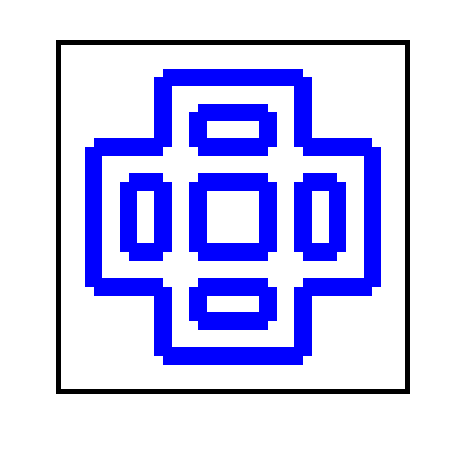
\includegraphics[width=\textwidth]{FinalFigures/defect_trio_1st_geo_b.pdf}
        \vspace{-1.3cm}
        \caption{}
        \label{fig:subfig-2}
    \end{subfigure}
    \begin{subfigure}{0.3\textwidth}
        \centering
        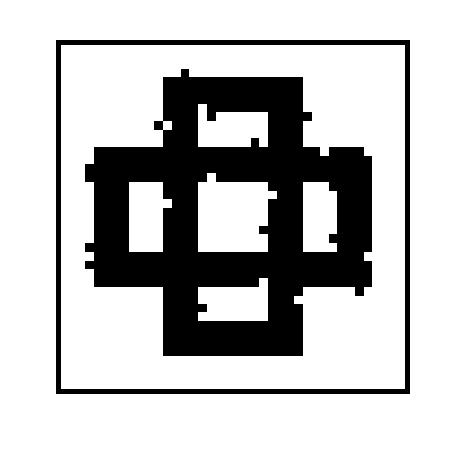
\includegraphics[width=\textwidth]{FinalFigures/defect_trio_1st_geo_c.pdf}
        \vspace{-1.3cm}
        \caption{}
        \label{fig:subfig-3}
    \end{subfigure}    
    \caption{a) the defect-free design geometry, b) edge pixels of the design geometry subject to random flipping, and c) a defective geometry after flipping a preset proportion of edge pixels.}
    \label{fig:defect_trio_1st_geo}
\end{figure}

For the three spectral projection ``sampling strategies'' (defined in \Cref{subsubsec:spectral projection}), the method parameters and corresponding number of sample points are shown in \Cref{table:7D_gamma_sampling_strategies}. Note that following a convergence study, the 10000 Monte Carlo sample set is taken to represent the ground truth for computing the true probability density function (PDF) of the output space (bandgap size and center location). The degree for the quadrature rule approach was set to be 2, since due to the exponential nature of the full tensor grid product, degree 3 or higher would require more points and computation than the 10000 MC samples and would thus be useless as a way to approximate the output space PDF. For the sparse grid approach, we look to maximize computational savings and so choose the lowest grid order as a comparison point.
\begin{table}[H]
    \centering
    \small
    \caption{Polynomial degree (PD) and number of sample points for each of the spectral projection methods}
    \label{table:7D_gamma_sampling_strategies}
    \begin{tabular}{ccc} 
        \toprule
        Sampling Method & Degree & Number of Points \\
        \midrule
        Monte Carlo & N/A & 100, 1000, 10000 \\
        Quadrature Rule & 1, 2 & 128, 2187 \\
        Sparse Grid & 1 & 15 \\
        \bottomrule
    \end{tabular}
\end{table}

For visualization purposes, some of the results of running the finite element model on the above Monte Carlo sampled datasets are shown in \Cref{fig:bgtbs_trio_hist_7d_gamma}. It would be difficult for the human eye to perceive the exact shape of the output distributions until some number of samples between $10^3$ or $10^4$, and so the purpose of this study is to see if the same output distribution shape can be captured for much fewer than $\sim 10^3$ samples via the UQ techniques.
% \begin{figure}[H]
% 	\centering 
% 	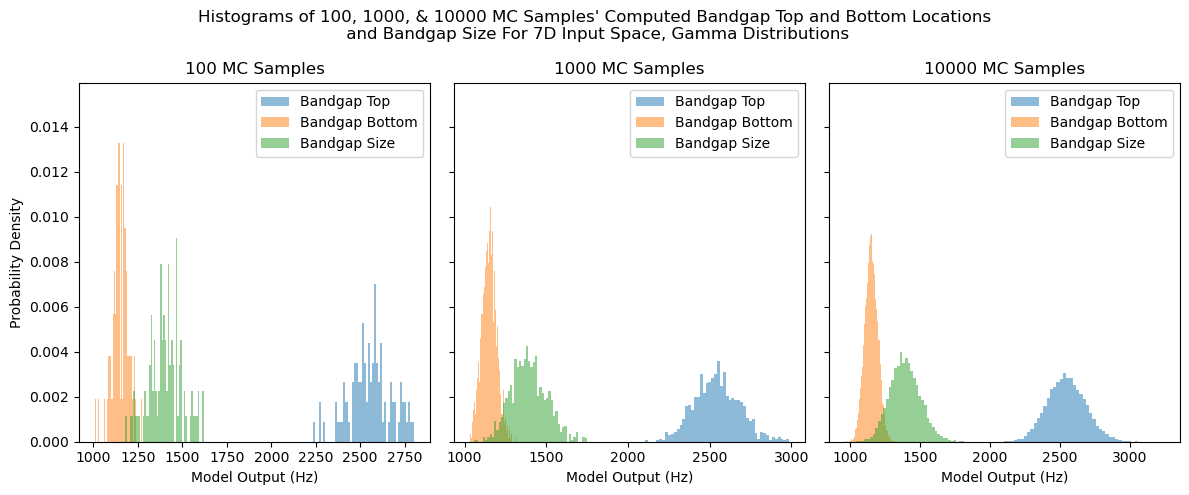
\includegraphics[width=\textwidth]{Figures/bgtbs_trio_hist_7d_gamma.png}	
% 	\caption{Histograms of the output variables for the Monte Carlo input datasets, band gap size and location, with location expressed in terms of bandgap top and bottom. Note that these two are combined later into the quantity bandgap center.} 
% 	\label{bgtbs_trio_hist_7d_gamma}%
% \end{figure}

\begin{figure}[H]
    \centering
    \begin{subfigure}{0.3\textwidth}
        \centering
        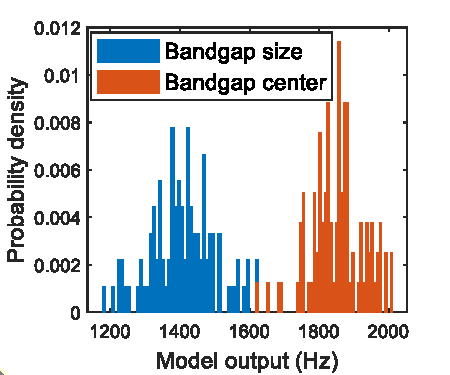
\includegraphics[width=\textwidth]{FinalFigures/bgtbs_trio_hist_7d_gamma_a.pdf}
        \caption{}
        \label{fig:subfig-1}
    \end{subfigure}\quad
    \begin{subfigure}{0.3\textwidth}
        \centering
        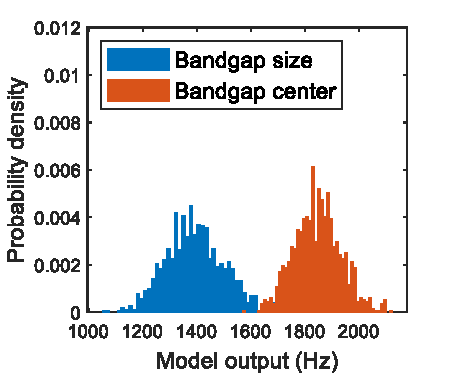
\includegraphics[width=\textwidth]{FinalFigures/bgtbs_trio_hist_7d_gamma_b.pdf}
        \caption{}
        \label{fig:subfig-2}
    \end{subfigure}\quad
    \begin{subfigure}{0.3\textwidth}
        \centering
        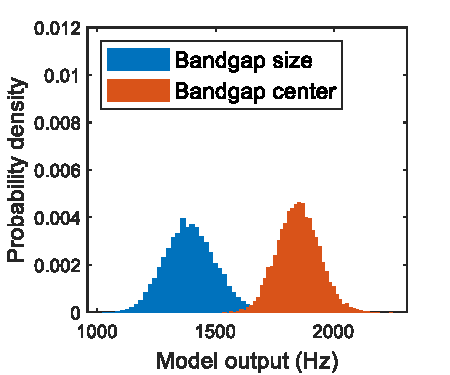
\includegraphics[width=\textwidth]{FinalFigures/bgtbs_trio_hist_7d_gamma_c.pdf}
        \caption{}
        \label{fig:subfig-3}
    \end{subfigure}    
    \caption{Histograms of FE outputs (bandgap size and center frequency) for a) 100, b) 1000, and c) 10000 Monte Carlo input samples. These histograms illustrate the data the UQ
surrogate models are ingesting and compared against.}
    \label{fig:bgtbs_trio_hist_7d_gamma}
\end{figure}

These outputs and inputs are then fed into PCE models for fitting. Only one set of representative fit results is shown in \Cref{fig:bgs_trio_hist_quad_fit_7d_gamma} for visualization purposes and brevity. The fit process for all the datasets in \Cref{table:7D_gamma_sampling_strategies} is the same and generates comparable results. The PCE surrogate fit however, will fail in cases where there are insufficient samples to fit all the polynomial coefficients (underdetermined problem), but usually does not suffer from overfitting issues as the PCE model does not aim to converge pointwise to the true model, instead only converging in probability distribution (as implied by the mean-square convergence). Figure 8 shows the performance of surrogate models constructed from 100 Monte Carlo samples compared with the baseline histograms of 100, 1000, and 10000 Monte Carlo samples. 
% \begin{figure}[H]
% 	\centering 
%         \begin{subfigure}[b]{\textwidth}
%             \centering 
%             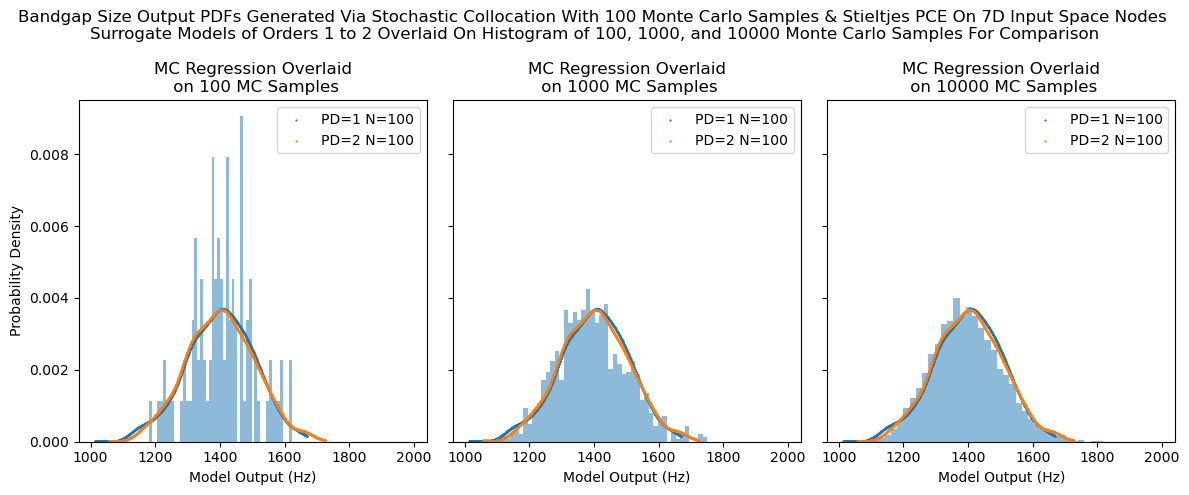
\includegraphics[width=\textwidth]{Figures/bgs_trio_hist_mc_fit_7d_n100_gamma.png}	    
%         \end{subfigure}
%         \begin{subfigure}[b]{\textwidth}
%             \centering
%             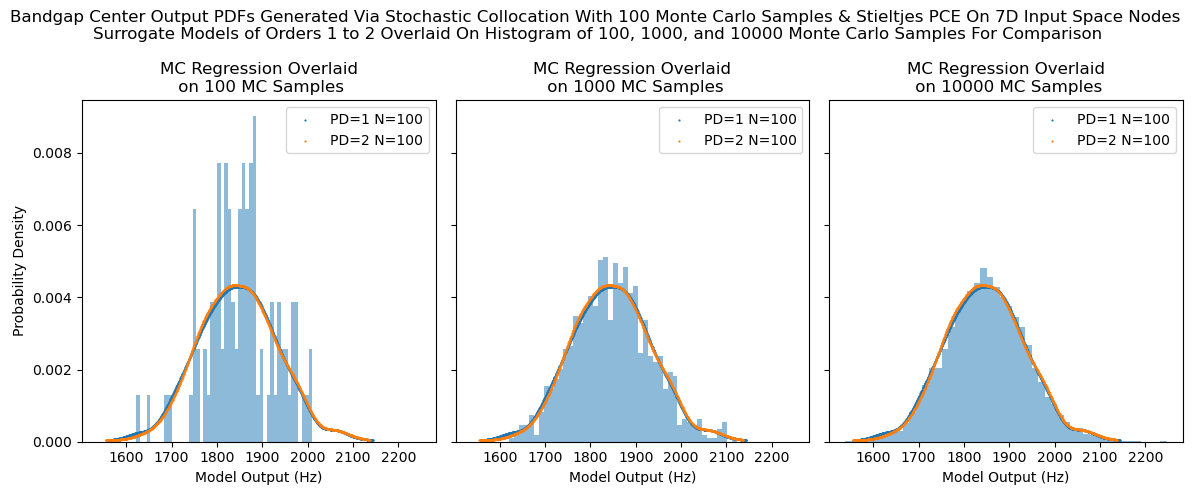
\includegraphics[width=\textwidth]{Figures/bgc_trio_hist_mc_fit_7d_n100_gamma.png}	    
%         \end{subfigure}
% 	\caption{Probability density functions of bandgap size and center from 1st and 2nd degree surrogate models constructed from 100 MC samples, overlaid on histograms of 100, 1000, and 10000 computed MC samples. The curves in each pane, which are generated with KDE on surrogate samples, are the same and it is only the background histograms that change. This indicates that with the same 100 samples as on the left plot panes, the PCE process was able to reconstruct a PDF that matches nearly perfectly to the 10000 sample ground truth.} 
% 	\label{fig:bgs_trio_hist_quad_fit_7d_gamma}%
% \end{figure}


\begin{figure}[H]
    \centering
    % \begin{subfigure}{0.3\textwidth}
    %     \centering
    %     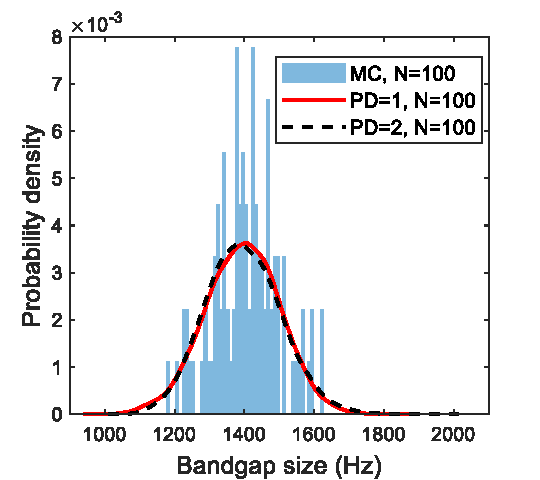
\includegraphics[width=\textwidth]{FinalFigures/bgs_trio_hist_mc_fit_7d_n100_gamma_a.pdf}
    %     \caption{}
    %     \label{fig:subfig-1}
    % \end{subfigure}\quad
    % \begin{subfigure}{0.3\textwidth}
    %     \centering
    %     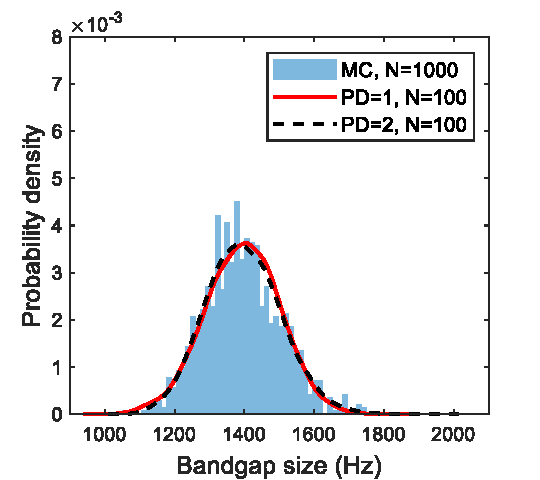
\includegraphics[width=\textwidth]{FinalFigures/bgs_trio_hist_mc_fit_7d_n100_gamma_b.pdf}
    %     \caption{}
    %     \label{fig:subfig-2}
    % \end{subfigure}\quad
    % \begin{subfigure}{0.3\textwidth}
    %     \centering
    %     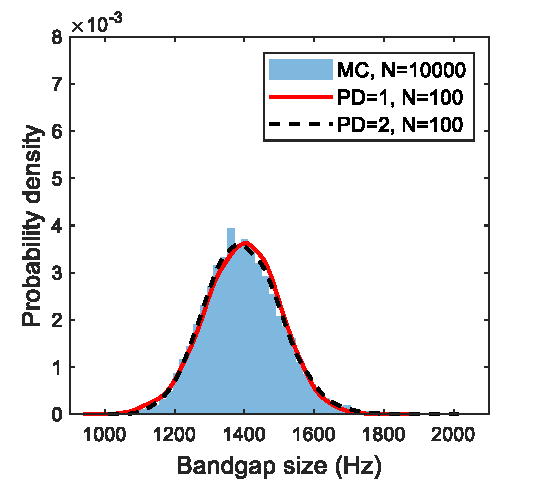
\includegraphics[width=\textwidth]{FinalFigures/bgs_trio_hist_mc_fit_7d_n100_gamma_c.pdf}
    %     \caption{}
    %     \label{fig:subfig-3}
    % \end{subfigure}
    
    % \vspace{0.5cm}
    
    % \begin{subfigure}{0.3\textwidth}
    %     \centering
    %     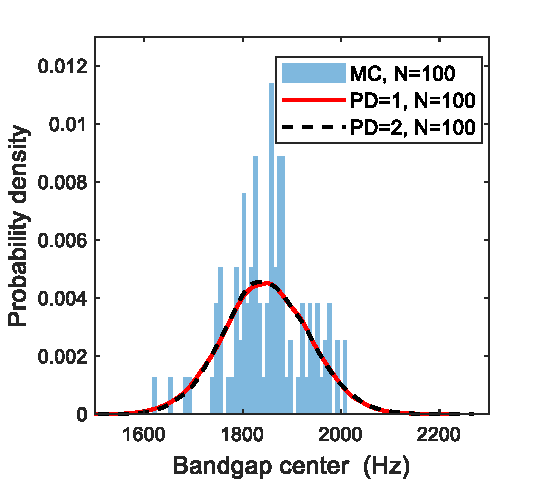
\includegraphics[width=\textwidth]{FinalFigures/bgc_trio_hist_mc_fit_7d_n100_gamma_a.pdf}
    %     \caption{}
    %     \label{fig:subfig-4}
    % \end{subfigure}\quad
    % \begin{subfigure}{0.3\textwidth}
    %     \centering
    %     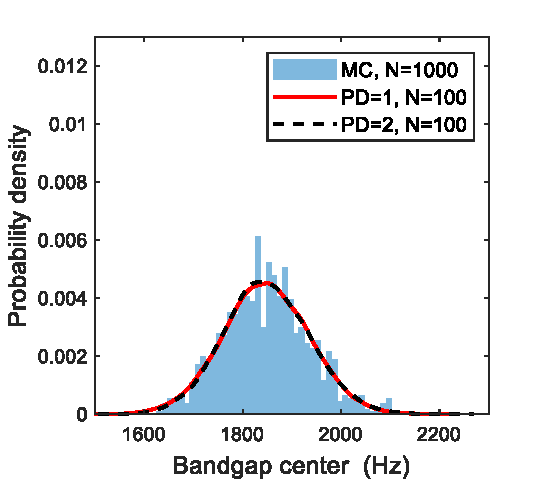
\includegraphics[width=\textwidth]{FinalFigures/bgc_trio_hist_mc_fit_7d_n100_gamma_b.pdf}
    %     \caption{}
    %     \label{fig:subfig-5}
    % \end{subfigure}\quad
    % \begin{subfigure}{0.3\textwidth}
    %     \centering
    %     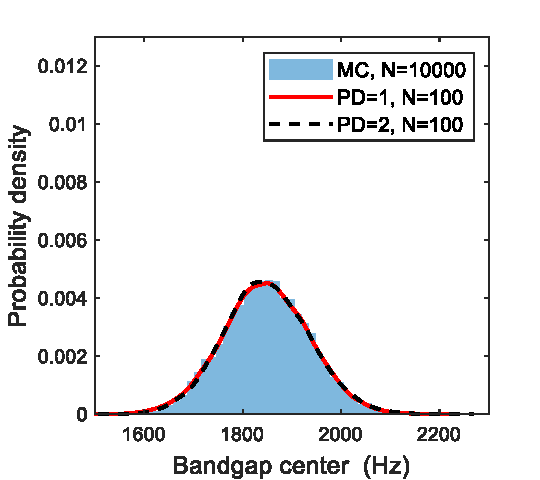
\includegraphics[width=\textwidth]{FinalFigures/bgc_trio_hist_mc_fit_7d_n100_gamma_c.pdf}
    %     \caption{}
    %     \label{fig:subfig-6}
    % \end{subfigure}

        \begin{subfigure}{0.93\textwidth}
        \centering
        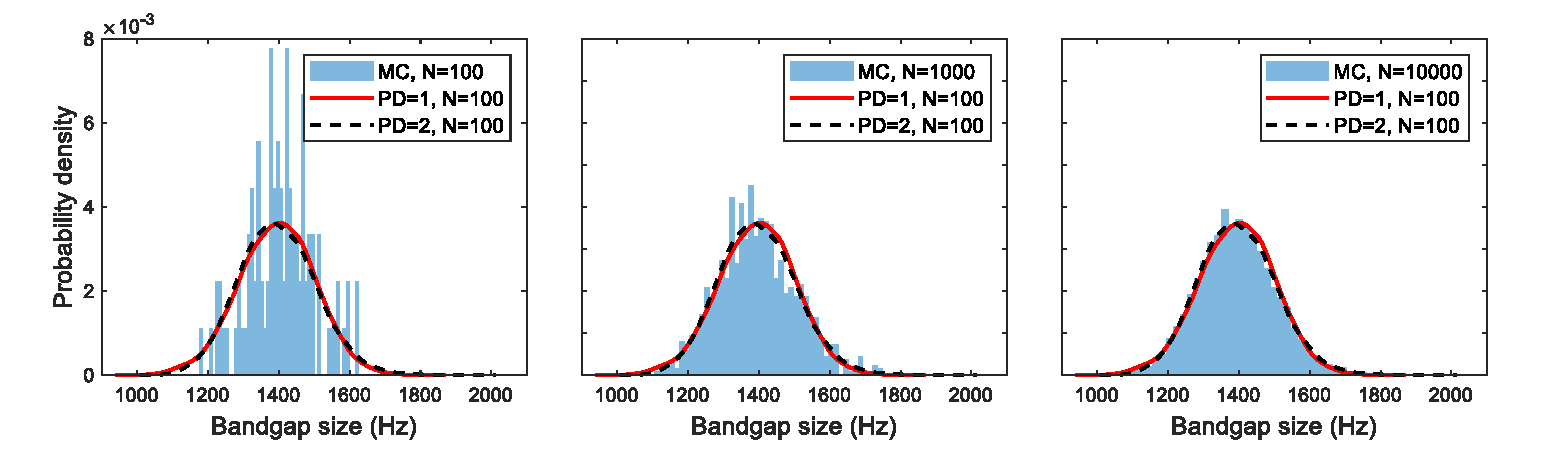
\includegraphics[width=\textwidth]{FinalFigures/bgs_trio_hist_mc_fit_7d_n100_gamma.pdf}
        \caption{}
        \label{fig:subfig-4}
    \end{subfigure}
    
    \vspace{0.5cm}
    
    \begin{subfigure}{0.93\textwidth}
        \centering
        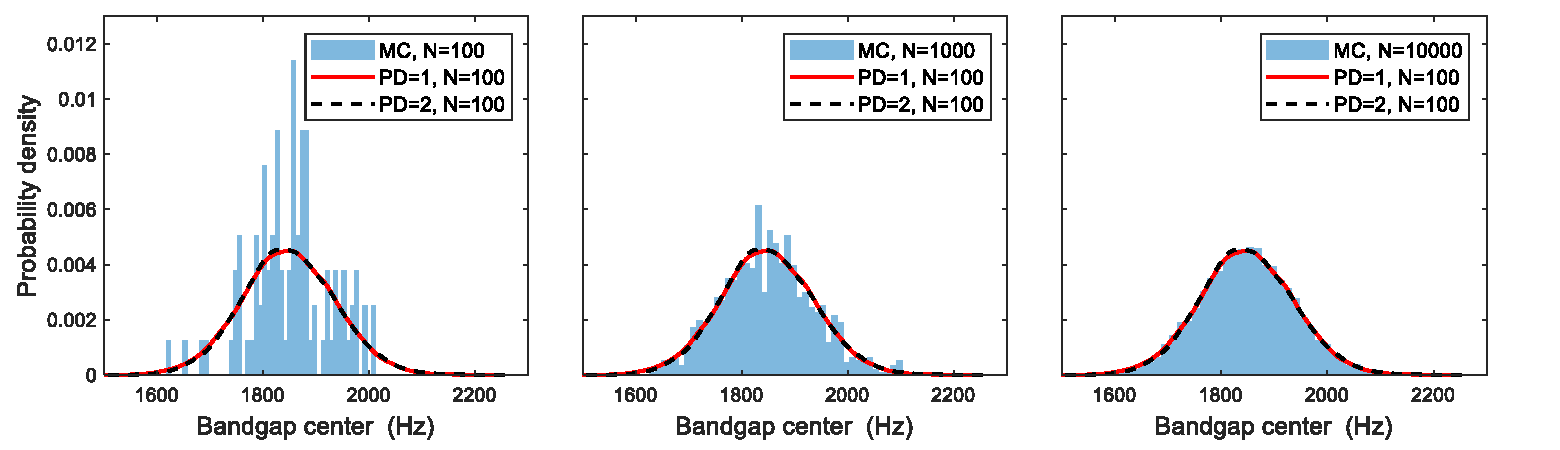
\includegraphics[width=\textwidth]{FinalFigures/bgc_trio_hist_mc_fit_7d_n100_gamma.pdf}
        \caption{}
        \label{fig:subfig-4}
    \end{subfigure}
    
    \caption{Probability density functions of a) bandgap size and b) center frequency from 1\textsuperscript{st} and 2\textsuperscript{nd} PCE degree surrogate models constructed from 100 Monte Carlo samples, overlaid on histograms of 100, 1000, and 10000 FE computed Monte Carlo samples. The curves in each pane are generated with kernel density estimation (KDE) on 1000 surrogate output samples and show the surrogate performance relative to the MC ground truth.}
    \label{fig:bgs_trio_hist_quad_fit_7d_gamma}
\end{figure}

In \Cref{fig:2d_hist_7d_input_pd1_quad_gamma} we compare the fit results of the three spectral projection sampling strategies and PCE surrogates with 10000 Monte Carlo computed samples which represents ground truth. The figure shows a heatmap of the existence of band gaps for the geometry shown in \Cref{fig:defect_trio_1st_geo} as the material properties and geometric defects are varied. One can see that with orders of magnitude fewer samples, we have very closely matched the probability distribution of the actual output space. Even the surrogate model fitted with just 15 sparse grid samples was able to faithfully represent, albeit with slight differences, the probability distribution of the output space. 
\begin{figure}[H]
    \centering
    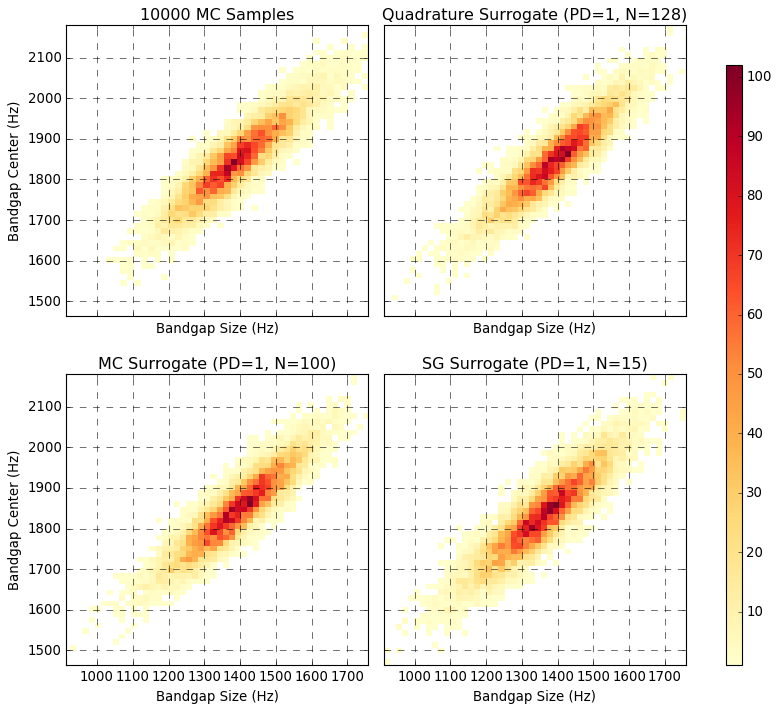
\includegraphics[width=\textwidth]{Figures/2d_hist_7d_input_pd1_quad_gamma.png}
    \caption{2D heatmaps of bandgap sizes and center locations. The 10000 Monte Carlo FE computed samples represents the ground truth. For comparison are the surrogate models trained on 128 quadrature rule samples, 100 Monte Carlo samples, and 15 sparse grid samples.} 
    \label{fig:2d_hist_7d_input_pd1_quad_gamma}
\end{figure}

% \begin{figure}[h]
%     \centering
%     \begin{subfigure}{0.36\textwidth}
%         \centering
%         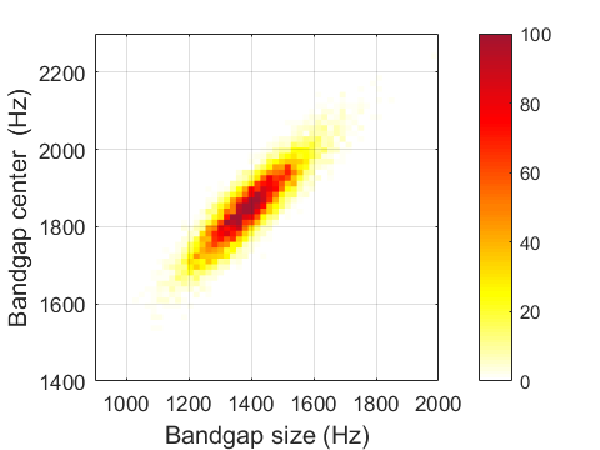
\includegraphics[width=\textwidth]{FinalFigures/2d_hist_7d_input_pd1_quad_gamma_a.pdf}
%         \caption{}
%         \label{fig:subfig-1}
%     \end{subfigure}
%     \begin{subfigure}{0.36\textwidth}
%         \centering
%         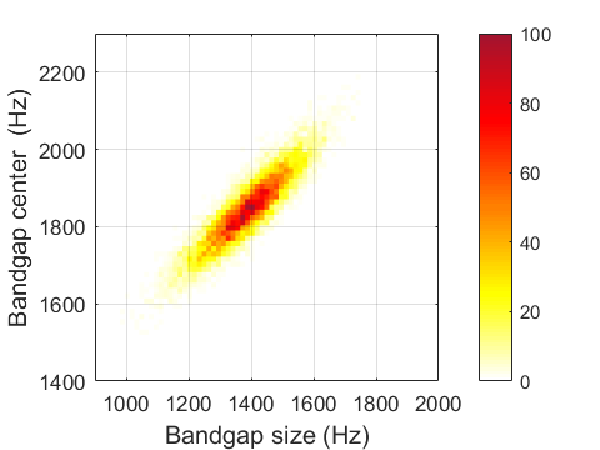
\includegraphics[width=\textwidth]{FinalFigures/2d_hist_7d_input_pd1_quad_gamma_b.pdf}
%         \caption{}
%         \label{fig:subfig-2}
%     \end{subfigure}
    
%     \vspace{0.5cm}
    
%     \begin{subfigure}{0.36\textwidth}
%         \centering
%         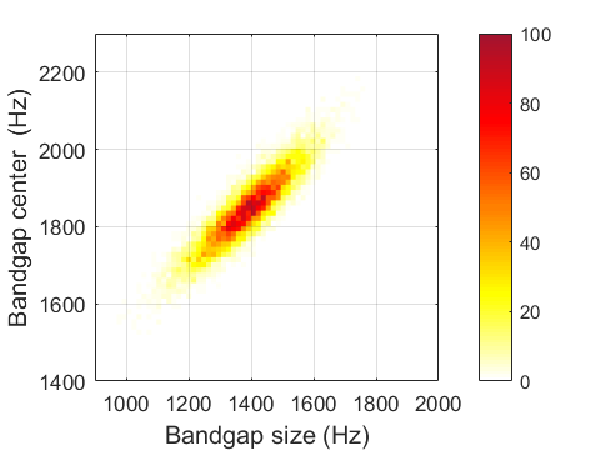
\includegraphics[width=\textwidth]{FinalFigures/2d_hist_7d_input_pd1_quad_gamma_c.pdf}
%         \caption{}
%         \label{fig:subfig-3}
%     \end{subfigure}
%     \begin{subfigure}{0.36\textwidth}
%         \centering
%         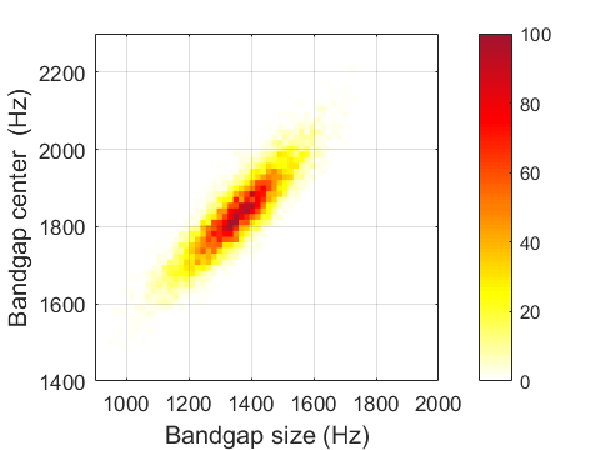
\includegraphics[width=\textwidth]{FinalFigures/2d_hist_7d_input_pd1_quad_gamma_d.pdf}
%         \caption{}
%         \label{fig:subfig-4}
%     \end{subfigure}
%         \caption{2D heatmaps of bandgap sizes and center frequency locations for a) ground truth constructed by 10000 Monte Carlo samples, b) 10000 samples drawn from the surrogate model constructed from quadrature rule sampling (128 samples), c) 10000 samples from the surrogate model constructed from PCE fit on 100 Monte Carlo samples, and d) 10000 samples from the surrogate model constructed from PCE fit on 15 sparse grid samples.}
% 	\label{fig:2d_hist_7d_input_pd1_quad_gamma}%    

%     \label{fig:2d_hist_7d_input_pd1_quad_gamma}
% \end{figure}

%%%%%%%%%%%%%%%%%%%%%%%%%%%%%%%%%%%%%%%%%%%%%%%%%%%%%%%%%%%%%%%%%%%%%%%%%%%%%%%%%%%%%%%%%%%%%%%%%%%%%%%%%%%%%%%%%%%
\subsection{7D Gaussian Input Space Study}
\label{subsec:7D Gaussian Input Space}
This study demonstrates the applicability of the spectral projection and PCE methods to a different set of distributions, with different material properties, and a different unit cell geometry. Like the previous study, the input space consists of six stochastic material properties and a geometry defect parameter. However unlike previously, all 7 inputs now have truncated normal distributions bounded by four standard deviations above and below the mean. This distribution choice represents another popular choice in the literature for representing material parameters and are detailed in \Cref{7D_Gaussian_Input_Table} and \Cref{fig:7d_input_mc_10000_2nd_geo}. The material properties have also been swapped in this study from bulk and shear moduli to their counterparts, the Young's Modulus and Poisson ratio, to demonstrate the generalizability of the UQ methods to choice of parameters. While the Young's Modulus numerically is on the same scale as the bulk and shear moduli (GPa and MPa for the stiff and soft materials respectively), the Poisson ratio is on a completely different scale, bounded between 0 and 0.5, and presents an opportunity to test if the UQ methods and software packages are robust to input distributions at vastly different scales, which in theory should be of no issue.

\begin{table}[H]
\centering
%\small
\tiny
\caption{7D Gaussian Input Space Material \& Geometry Property Distributions and Parameters}
\label{7D_Gaussian_Input_Table}
\begin{tabularx}{\linewidth}{Xccccc} 
\toprule
Material Property & Distribution & Mean ($\mu$) & Standard Deviation ($\sigma$) & Lower Trunc. & Upper Trunc. \\
\midrule
\( \text{Soft Young's Modulus } (E_{Soft})\) & \( \text{Truncated Normal} \) & \( 200 \text{ MPa} \) & \( 0.08\mu \) & \( -4\sigma \) & \( 4\sigma \) \\
\( \text{Stiff Young's Modulus } (E_{Stiff})\) & \( \text{Truncated Normal} \) & \( 200 \text{ GPa} \) & \( 0.02\mu \) & \( -4\sigma \) & \( 4\sigma \) \\
\( \text{Soft density } (\rho_{Soft})\) & \( \text{Truncated Normal} \) & \( 1000 \text{ kg/m$^3$} \) & \( 0.08\mu \) & \( -4\sigma \) & \( 4\sigma \) \\
\( \text{Stiff density } (\rho_{Stiff})\) & \( \text{Truncated Normal} \) & \( 8000 \text{ kg/m$^3$} \) & \( 0.02\mu \) & \( -4\sigma \) & \( 4\sigma \) \\
\( \text{Soft Poisson ratio } (\nu_{Soft})\) & \( \text{Truncated Normal} \) & \( 0.38 \) & \( 0.02\mu \) & \( -4\sigma \) & \( 4\sigma \) \\
\( \text{Stiff Poisson ratio } (\nu_{Stiff})\) & \( \text{Truncated Normal} \) & \( 0.28 \) & \( 0.02\mu \) & \( -4\sigma \) & \( 4\sigma \) \\
\( \text{Geometry flip proportion }  (FP)\) & \( \text{Truncated Normal} \) & \( 0.025 \) & \( 0.08\mu \) & \( -4\sigma \) & \( 4\sigma \) \\
\bottomrule
\end{tabularx}
\end{table}

% \begin{figure}[H]
% 	\centering 
% 	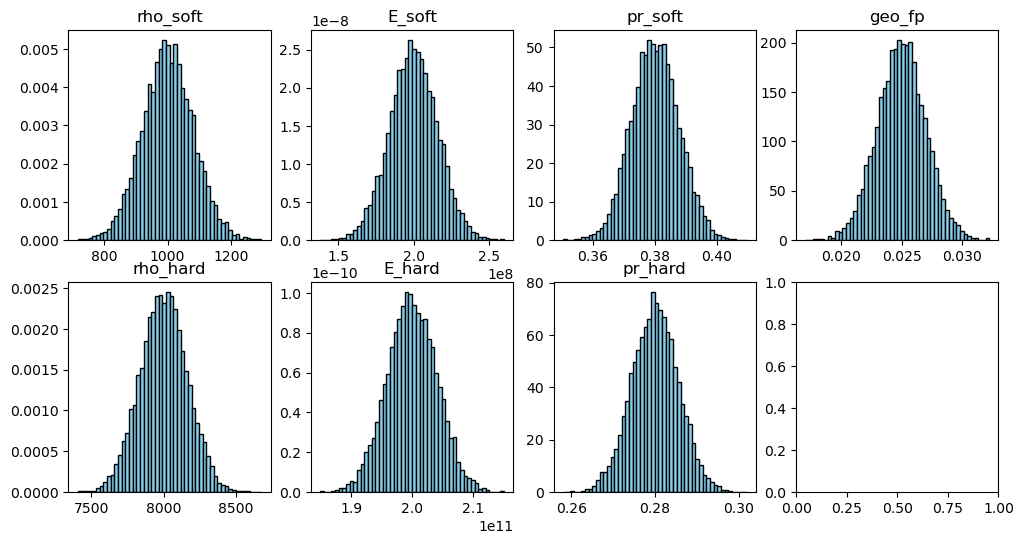
\includegraphics[width=\textwidth]{Figures/P_7d_input_mc_10000_2nd_geo.png}	
% 	\caption{10000 Monte Carlo samples of the 7D Gaussian input space, for visualization of the input space distribution shapes.} 
% 	\label{fig:7d_input_mc_10000_2nd_geo}%
% \end{figure}

\begin{figure}[H]
    \centering
    \begin{subfigure}{0.24\textwidth}
        \centering
        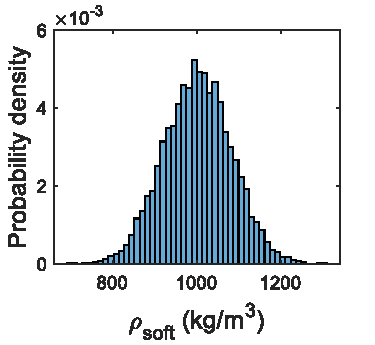
\includegraphics[width=\textwidth]{FinalFigures/P_7d_input_mc_10000_2nd_geo_a.pdf}
        \caption{}
        \label{fig:subfig-1}
    \end{subfigure}
    \hspace{0.02\textwidth}
    \begin{subfigure}{0.24\textwidth}
        \centering
        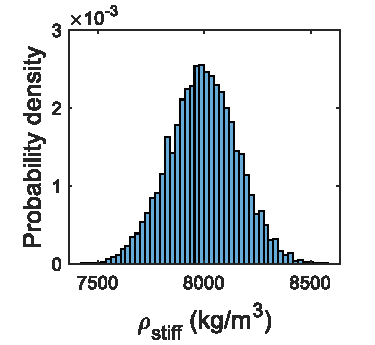
\includegraphics[width=\textwidth]{FinalFigures/P_7d_input_mc_10000_2nd_geo_b.pdf}
        \caption{}
        \label{fig:subfig-2}
    \end{subfigure}
    \hspace{0.02\textwidth}
    \begin{subfigure}{0.24\textwidth}
        \centering
        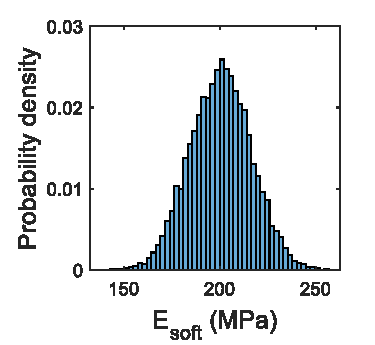
\includegraphics[width=\textwidth]{FinalFigures/P_7d_input_mc_10000_2nd_geo_c.pdf}
        \caption{}
        \label{fig:subfig-3}
    \end{subfigure}
    
    \medskip
    
    \begin{subfigure}{0.24\textwidth}
        \centering
        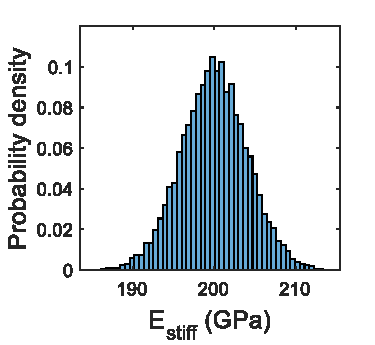
\includegraphics[width=\textwidth]{FinalFigures/P_7d_input_mc_10000_2nd_geo_d.pdf}
        \caption{}
        \label{fig:subfig-4}
    \end{subfigure}
    \hfill
    \begin{subfigure}{0.24\textwidth}
        \centering
        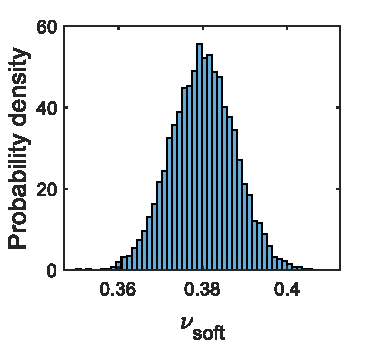
\includegraphics[width=\textwidth]{FinalFigures/P_7d_input_mc_10000_2nd_geo_e.pdf}
        \caption{}
        \label{fig:subfig-5}
    \end{subfigure}
    \hfill
    \begin{subfigure}{0.24\textwidth}
        \centering
        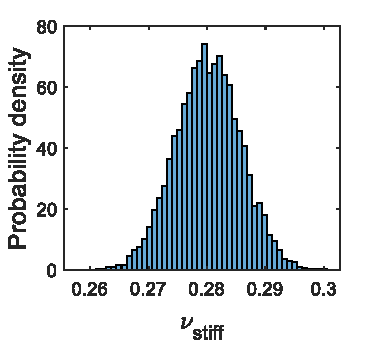
\includegraphics[width=\textwidth]{FinalFigures/P_7d_input_mc_10000_2nd_geo_f.pdf}
        \caption{}
        \label{fig:subfig-6}
    \end{subfigure}
    \hfill
    \begin{subfigure}{0.24\textwidth}
        \centering
        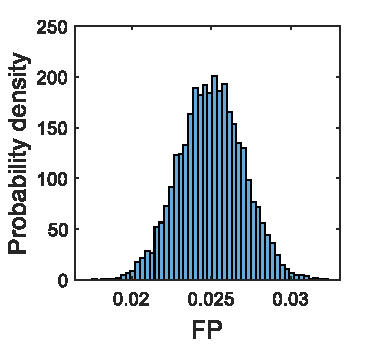
\includegraphics[width=\textwidth]{FinalFigures/P_7d_input_mc_10000_2nd_geo_g.pdf}
        \caption{}
        \label{fig:subfig-7}
    \end{subfigure}    
    \caption{10000 Monte Carlo samples of the 7D Gaussian input space, for visualization of the input space distribution shapes for a) density of the soft material, b) density of the stiff material, c) Young's modulus of the soft material, d) Young's modulus of the stiff material, e) Poisson ratio of the soft material, f) Poisson ratio of the stiff material, and g) flip proportion parameter for generating geometry defects.}
    \label{fig:7d_input_mc_10000_2nd_geo}
\end{figure}

Like before, the sampled geometry FP parameters are used to randomly generate defective geometries to pair with each set of sampled material properties. The typical process and result of the geometry defect generation process is shown in \Cref{fig:defect_trio_2nd_geo}.
% \begin{figure}[H]
% 	\centering 
% 	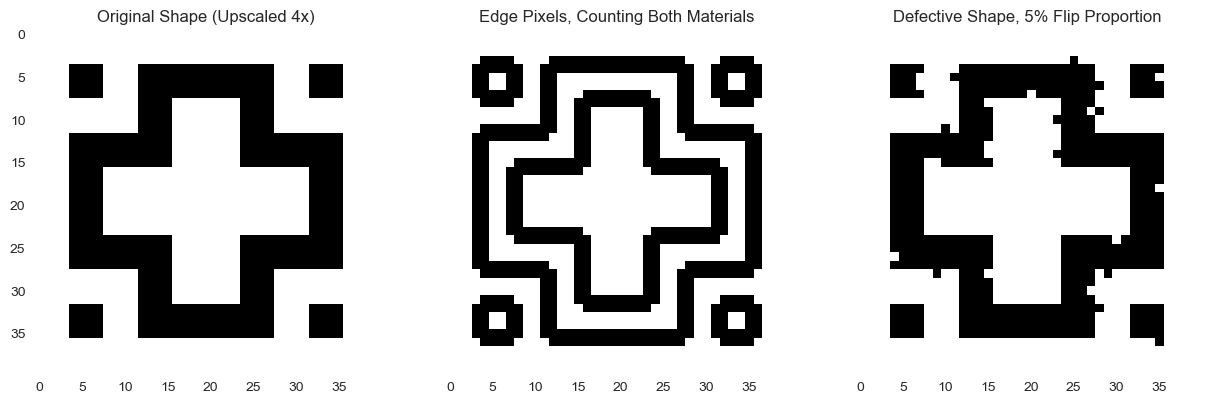
\includegraphics[width=\textwidth]{Figures/defect_trio_2nd_geo.png}	
% 	\caption{Left: The defect free designed geometry, scaled up to 40px by 40px. Center: edge pixels of the design geometry, which will be subjected to random flipping at preset proportion of the FP parameter. Right: one resulting defective geometry after flipping the preset proportion of the edge pixels. Note that this is a representative defect and that different randomly generated defects are (likely) used in each set of sample inputs.} 
% 	\label{defect_trio_2nd_geo}%
% \end{figure}

\begin{figure}[H]
    \centering
    \begin{subfigure}{0.3\textwidth}
        \centering
        
\includegraphics[width=\textwidth]{FinalFigures/defect_trio_2nd_geo_a.pdf}
        \vspace{-1.3cm}
        \caption{}
        \label{fig:subfig-1}
    \end{subfigure}
    \begin{subfigure}{0.3\textwidth}
        \centering
        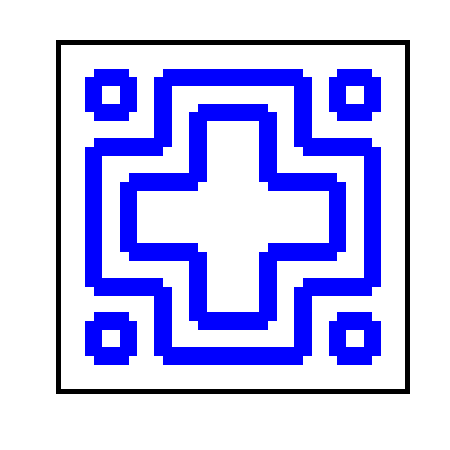
\includegraphics[width=\textwidth]{FinalFigures/defect_trio_2nd_geo_b.pdf}
        \vspace{-1.3cm}
        \caption{}
        \label{fig:subfig-2}
    \end{subfigure}
    \begin{subfigure}{0.3\textwidth}
        \centering
        
\includegraphics[width=\textwidth]{FinalFigures/defect_trio_2nd_geo_c.pdf}
        \vspace{-1.3cm}
        \caption{}
        \label{fig:subfig-3}
    \end{subfigure}    
    \caption{a) the defect-free design geometry, b) edge pixels of the design geometry subject to random flipping, and c) a defective geometry after flipping a preset 5\% proportion of the edge pixels.}
    \label{fig:defect_trio_2nd_geo}
\end{figure}

The three spectral projection sampling strategies, shown in \Cref{table:7D_gauss_sampling_strategies} are the same as in the previous study. Like before, the 10000 Monte Carlo sample set is taken to represent the ground truth for computing the true probability density function (PDF) of the output space (bandgap size and center location).

\begin{table}[H]
    \centering
    \small
    \caption{Polynomial degree and sample points for each of the spectral projection methods}
    \label{table:7D_gauss_sampling_strategies}
    \begin{tabular}{ccc} 
        \toprule
        Sampling Method & Degree & Number of Points \\
        \midrule
        Monte Carlo & N/A & 100, 1000, 10000 \\
        Quadrature Rule & 1, 2 & 128, 2187 \\
        Sparse Grid & 1 & 15 \\
        \bottomrule
    \end{tabular}
\end{table}

For visualization purposes, some of the results of running the finite element model on the above Monte Carlo sampled datasets are shown in \Cref{fig:bgtbs_trio_hist_7d_gaussian_2nd_geo}. Like previously, it is difficult for the human eye to perceive the exact shape of the output distributions until sample number reaches somewhere near $10^3$ or $10^4$, and so we try again to see if the true output distribution shape can be captured for much fewer than $\sim 10^3$ samples.
% \begin{figure}[H]
% 	\centering 
% 	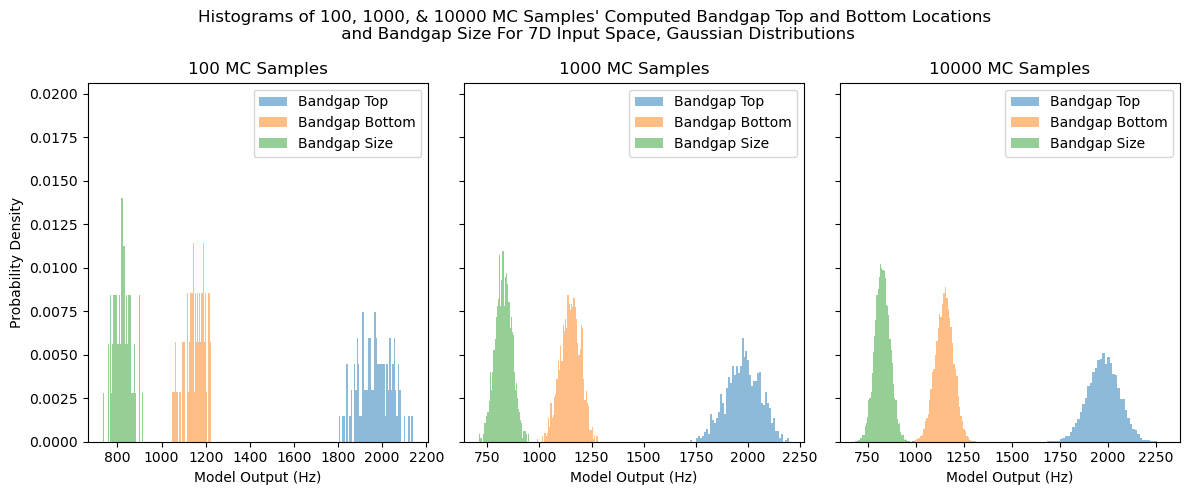
\includegraphics[width=\textwidth]{Figures/bgtbs_trio_hist_7d_gaussian_2nd_geo.png}	
% 	\caption{Histograms of the output variables for the Monte Carlo input datasets, band gap size and location, with location expressed in terms of bandgap top and bottom. Note that these two are combined later into the quantity bandgap center.} 
% 	\label{fig:bgtbs_trio_hist_7d_gaussian_2nd_geo}%
% \end{figure}

\begin{figure}[H]
    \centering
    \begin{subfigure}{0.3\textwidth}
        \centering
        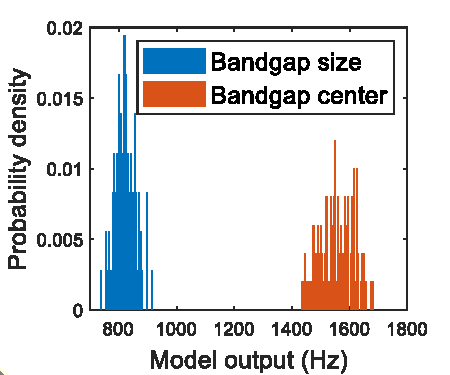
\includegraphics[width=\textwidth]{FinalFigures/bgtbs_trio_hist_7d_gaussian_2nd_geo_a.pdf}
        \caption{}
        \label{fig:subfig-1}
    \end{subfigure}\quad
    \begin{subfigure}{0.3\textwidth}
        \centering
        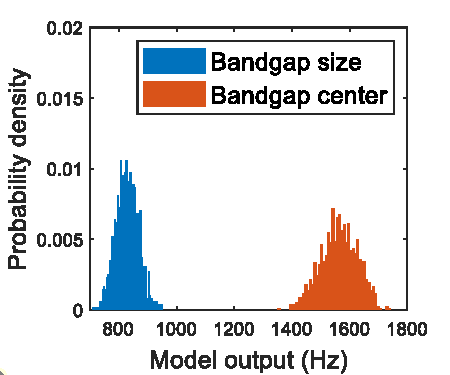
\includegraphics[width=\textwidth]{FinalFigures/bgtbs_trio_hist_7d_gaussian_2nd_geo_b.pdf}
        \caption{}
        \label{fig:subfig-2}
    \end{subfigure}\quad
    \begin{subfigure}{0.3\textwidth}
        \centering
        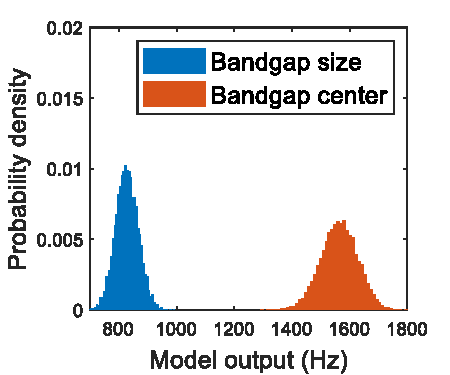
\includegraphics[width=\textwidth]{FinalFigures/bgtbs_trio_hist_7d_gaussian_2nd_geo_c.pdf}
        \caption{}
        \label{fig:subfig-3}
    \end{subfigure}    
    \caption{Histograms of the FE outputs (bandgap size and center frequency) for a) 100, b) 1000, c) 10000 Monte Carlo input samples. These histograms illustrate the data the UQ surrogate models are ingesting and compared against.}
    \label{fig:bgtbs_trio_hist_7d_gaussian_2nd_geo}
\end{figure}

These outputs and inputs are fed into PCE models for fitting, which similar to the previous study in \Cref{subsec:7D Gamma Input Space}, produced very similar results for each dataset, so for the purpose of visualization and brevity, only one set of representative surrogate fit results are shown in \Cref{fig:bgs_trio_hist_quad_fit_7d_2nd_geo}. The figure shows the performance of surrogate models constructed from 128 and 2187 quadrature rule samples compared with the baseline histograms of 100, 1000, and 10000 Monte Carlo samples. 
% \begin{figure}[H]
% 	\centering 
%         \begin{subfigure}[b]{\textwidth}
%             \centering 
%             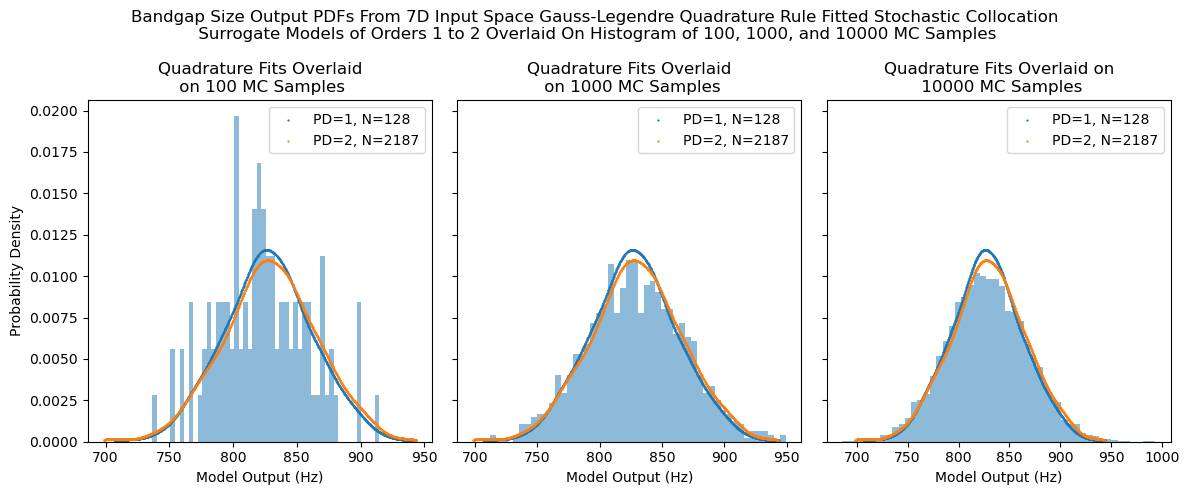
\includegraphics[width=\textwidth]{Figures/bgs_trio_hist_quad_fit_7d_2nd_geo.png}	    
%         \end{subfigure}
%         \begin{subfigure}[b]{\textwidth}
%             \centering
%             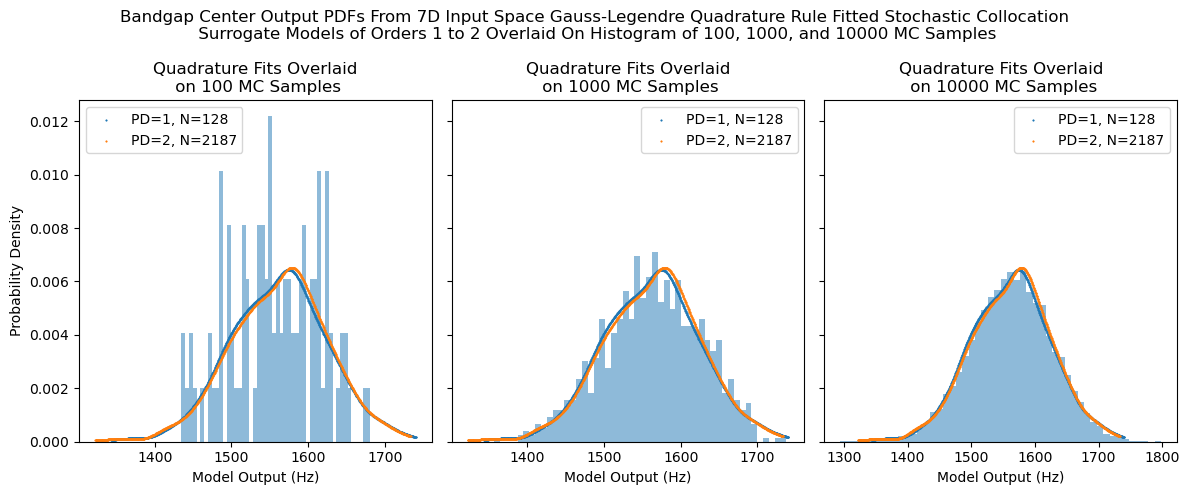
\includegraphics[width=\textwidth]{Figures/bgc_trio_hist_quad_fit_7d_2nd_geo.png}	    
%         \end{subfigure}
% 	\caption{Probability density functions of bandgap size and center from 1st and 2nd degree surrogate models constructed from 1st and 2nd order quadrature rule samples (128 \& 2187 samples respectively), overlaid on histograms of 100, 1000, and 10000 computed MC samples. Note that the curves in each pane, which are generated with KDE on surrogate samples, are the same and it is only the background histograms that change. We can infer that the 2nd order quadrature rule sampling is not necessary as it has a very similar PDF to the 1st order surrogate, which for 128 samples, appears to match the true PDF very closely.} 
% 	\label{fig:bgs_trio_hist_quad_fit_7d_2nd_geo}%
% \end{figure}

\begin{figure}[H]
    \centering
    % \begin{subfigure}{0.3\textwidth}
    %     \centering
    %     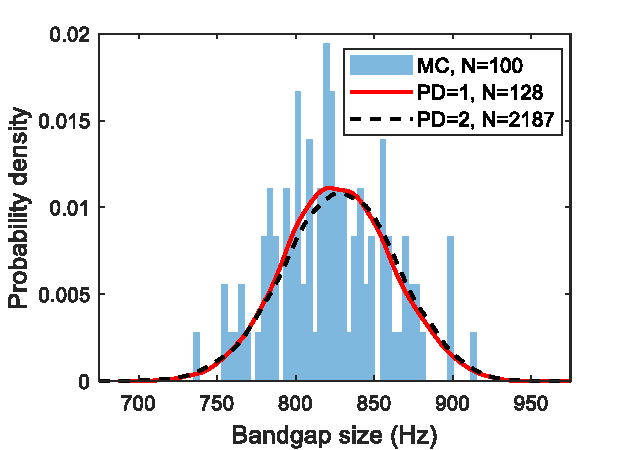
\includegraphics[width=\textwidth]{FinalFigures/bgs_trio_hist_quad_fit_7d_2nd_geo_a.pdf}
    %     \caption{}
    %     \label{fig:subfig-1}
    % \end{subfigure}\quad
    % \begin{subfigure}{0.3\textwidth}
    %     \centering
    %     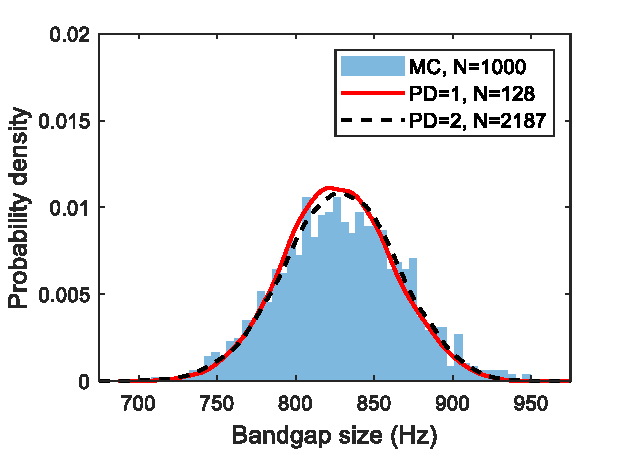
\includegraphics[width=\textwidth]{FinalFigures/bgs_trio_hist_quad_fit_7d_2nd_geo_b.pdf}
    %     \caption{}
    %     \label{fig:subfig-2}
    % \end{subfigure}\quad
    % \begin{subfigure}{0.3\textwidth}
    %     \centering
    %     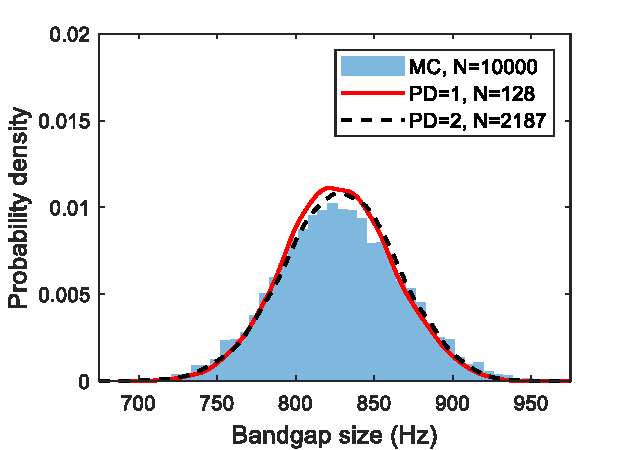
\includegraphics[width=\textwidth]{FinalFigures/bgs_trio_hist_quad_fit_7d_2nd_geo_c.pdf}
    %     \caption{}
    %     \label{fig:subfig-3}
    % \end{subfigure}
    
    % \vspace{0.5cm}
    
    % \begin{subfigure}{0.3\textwidth}
    %     \centering
    %     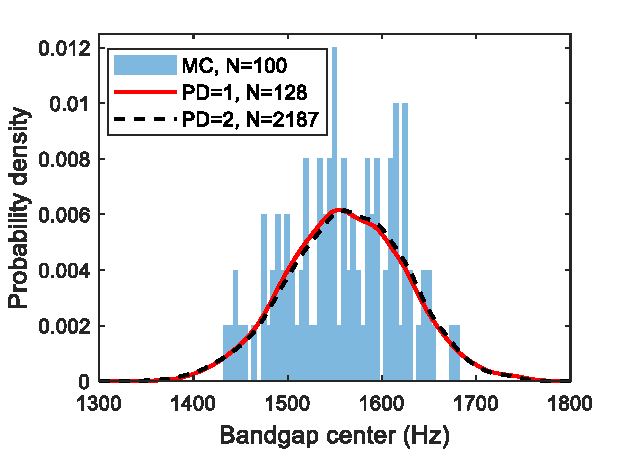
\includegraphics[width=\textwidth]{FinalFigures/bgc_trio_hist_quad_fit_7d_2nd_geo_a.pdf}
    %     \caption{}
    %     \label{fig:subfig-4}
    % \end{subfigure}\quad
    % \begin{subfigure}{0.3\textwidth}
    %     \centering
    %     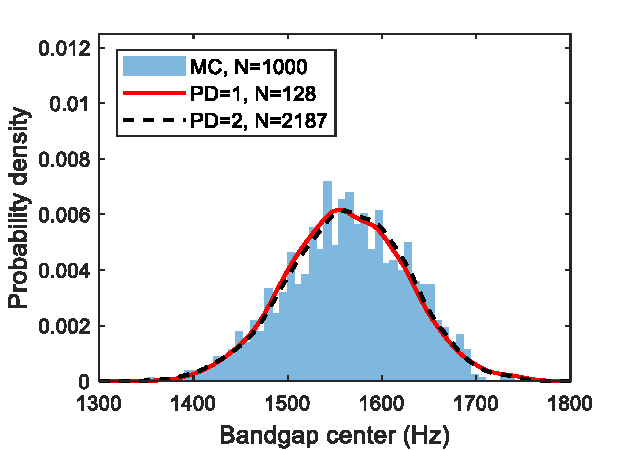
\includegraphics[width=\textwidth]{FinalFigures/bgc_trio_hist_quad_fit_7d_2nd_geo_b.pdf}
    %     \caption{}
    %     \label{fig:subfig-5}
    % \end{subfigure}\quad
    % \begin{subfigure}{0.3\textwidth}
    %     \centering
    %     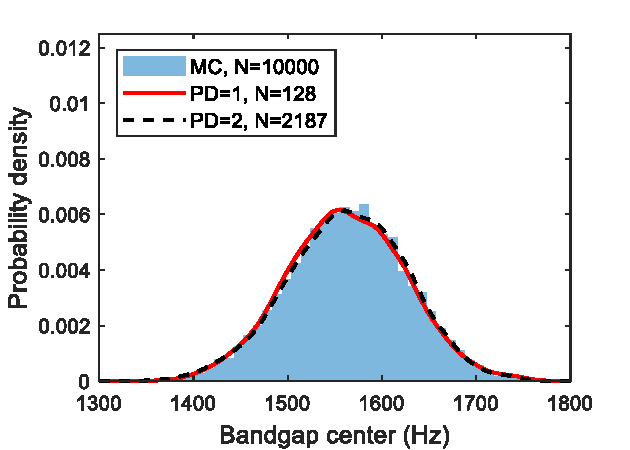
\includegraphics[width=\textwidth]{FinalFigures/bgc_trio_hist_quad_fit_7d_2nd_geo_c.pdf}
    %     \caption{}
    %     \label{fig:subfig-6}
    % \end{subfigure}
    
    \begin{subfigure}{\textwidth}
        \centering
        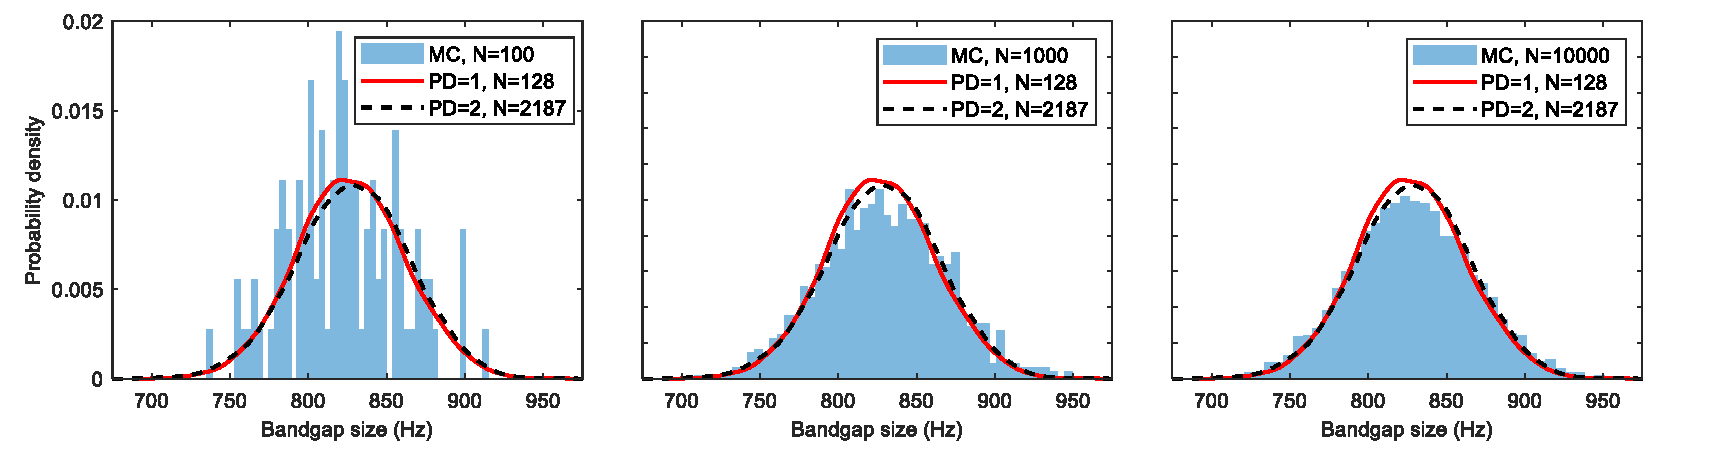
\includegraphics[width=\textwidth]{FinalFigures/bgs_trio_hist_quad_fit_7d_2nd_geo.pdf}
        \caption{}
        \label{fig:subfig-4}
    \end{subfigure}
    
    \vspace{0.5cm}
    
    \begin{subfigure}{\textwidth}
        \centering
        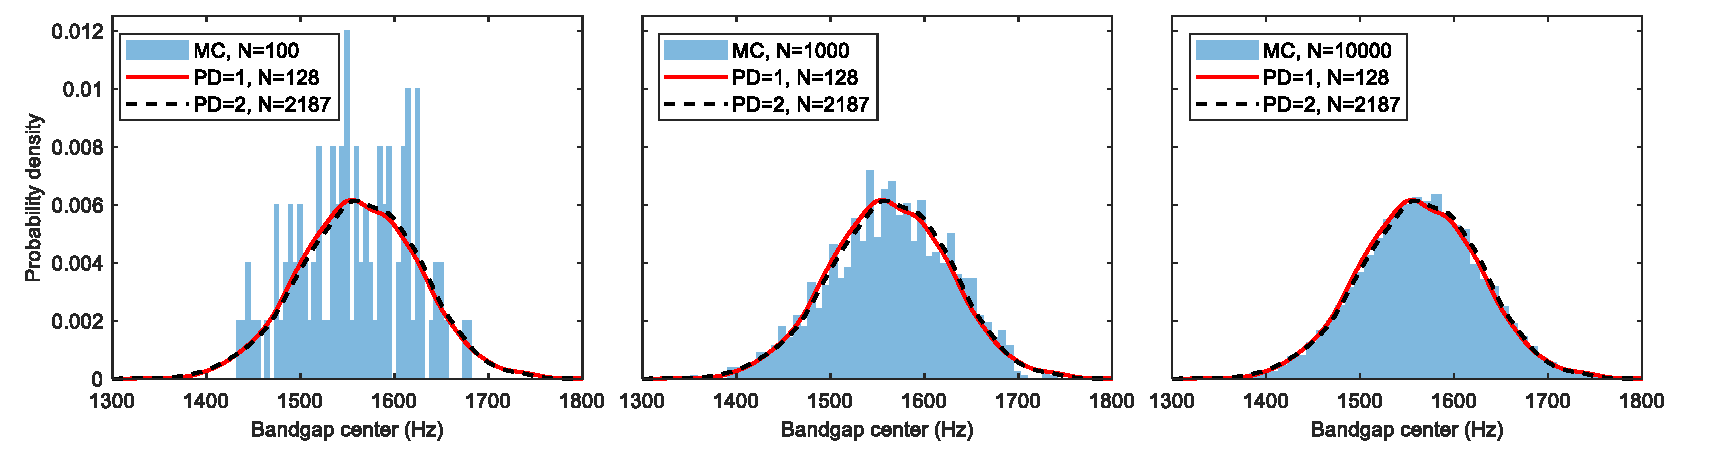
\includegraphics[width=\textwidth]{FinalFigures/bgc_trio_hist_quad_fit_7d_2nd_geo.pdf}
        \caption{}
        \label{fig:subfig-4}
    \end{subfigure}
    
    \caption{Probability density functions of a) bandgap size and b) center frequency from 1\textsuperscript{st} and 2\textsuperscript{nd} degree PCE surrogate models constructed from 1\textsuperscript{st} and 2\textsuperscript{nd} order quadrature rule sampling (128 and 2187 samples respectively), overlaid on histograms of 100, 1000, and 10000 computed MC samples. KDE curves in each pane are generated on 1000 surrogate model outputs and show the surrogate performance relative to the MC ground truth.}
    \label{fig:bgs_trio_hist_quad_fit_7d_2nd_geo}
\end{figure}

In \Cref{fig:2d_hist_7d_input_pd1_quad_2nd_geo}, we compare the fit results of the three spectral projection sampling strategies and their PCE surrogates with 10000 Monte Carlo computed samples which represents ground truth. Like with the previous study, the probability distribution of the actual output space is closely matched by the surrogate models fitted on order(s) of magnitude fewer samples. The sparse grid surrogate, using only 15 points, deviates further from the true distribution than the previous study, but is still reasonably good at about 12.5\% wider spread in the domain on both outputs.
\begin{figure}[H]
    \centering
    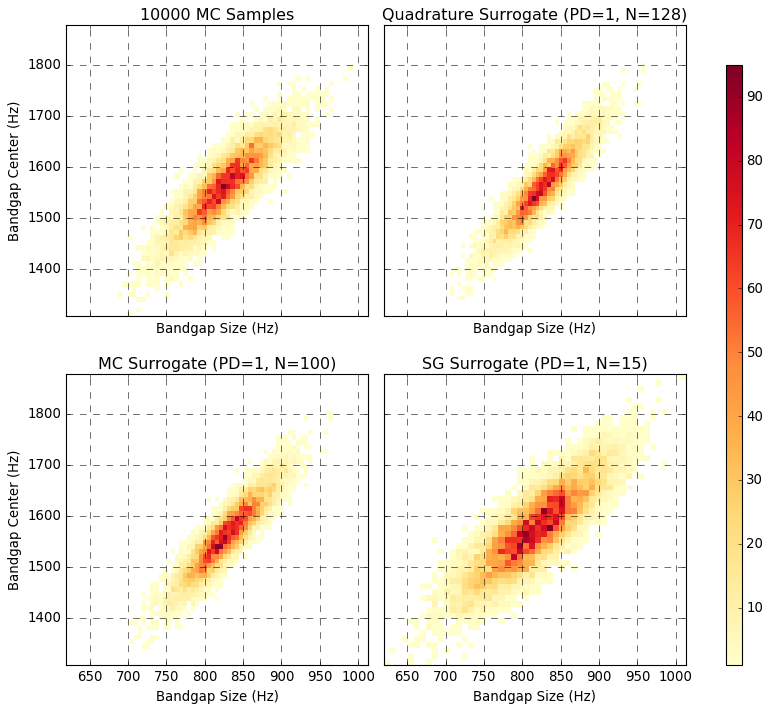
\includegraphics[width=\textwidth]{Figures/2d_hist_7d_input_pd1_quad_2nd_geo.png}	
    \caption{2D heatmaps of bandgap sizes and center locations. The 10000 Monte Carlo FE computed samples represents the ground truth. For comparison are the surrogate models trained on 128 quadrature rule samples, 100 Monte Carlo samples, and 15 sparse grid samples.} 
    \label{fig:2d_hist_7d_input_pd1_quad_2nd_geo}
\end{figure}

% \begin{figure}[H]
%     \centering
%     \begin{subfigure}{0.36\textwidth}
%         \centering
%         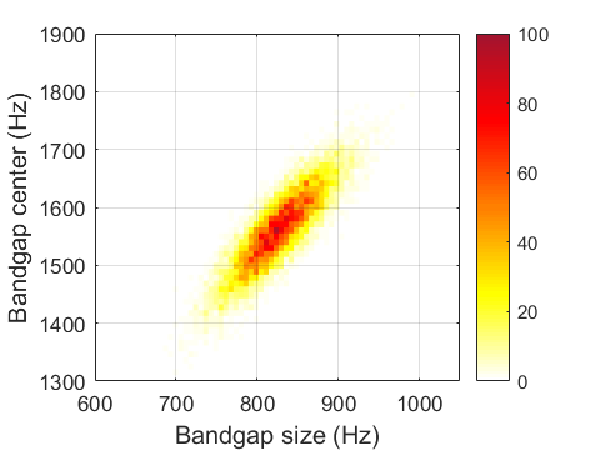
\includegraphics[width=\textwidth]{FinalFigures/2d_hist_7d_input_pd1_quad_2nd_geo_a.pdf}
%         \caption{}
%         \label{fig:subfig-1}
%     \end{subfigure}
%     \begin{subfigure}{0.36\textwidth}
%         \centering
%         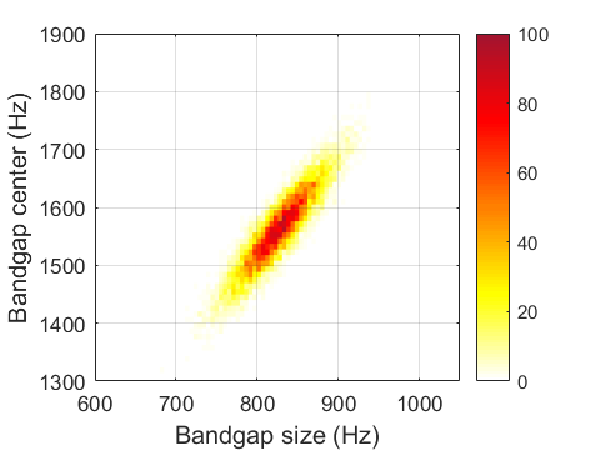
\includegraphics[width=\textwidth]{FinalFigures/2d_hist_7d_input_pd1_quad_2nd_geo_b.pdf}
%         \caption{}
%         \label{fig:subfig-2}
%     \end{subfigure}
    
%     \vspace{0.5cm}
    
%     \begin{subfigure}{0.36\textwidth}
%         \centering
%         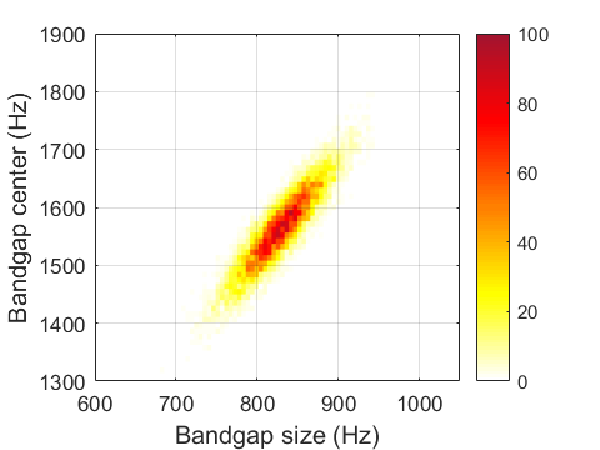
\includegraphics[width=\textwidth]{FinalFigures/2d_hist_7d_input_pd1_quad_2nd_geo_c.pdf}
%         \caption{}
%         \label{fig:subfig-3}
%     \end{subfigure}
%     \begin{subfigure}{0.36\textwidth}
%         \centering
%         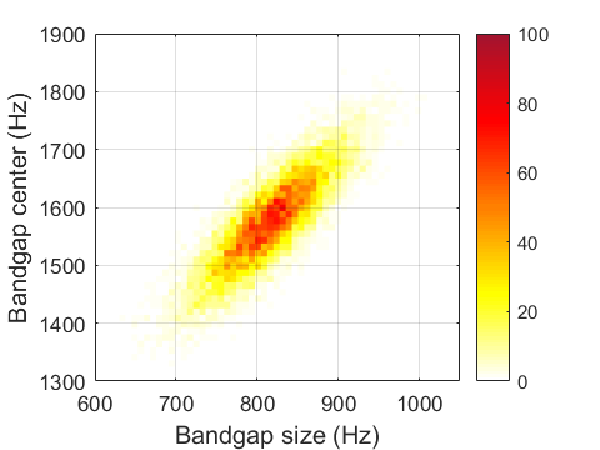
\includegraphics[width=\textwidth]{FinalFigures/2d_hist_7d_input_pd1_quad_2nd_geo_d.pdf}
%         \caption{}
%         \label{fig:subfig-4}
%     \end{subfigure}
%         \caption{2D color maps of bandgap sizes and center frequency locations for a) ground truth constructed by 10000 Monte Carlo samples, b) 10000 samples drawn from the surrogate model constructed from quadrature rule sampling (128 samples), c) 10000 samples from the surrogate model constructed from PCE fit on 100 Monte Carlo samples, and d) 10000 samples from the surrogate model constructed from PCE fit on 15 sparse grid samples.}
%     \label{fig:2d_hist_7d_input_pd1_quad_2nd_geo}
% \end{figure}

%%%%%%%%%%%%%%%%%%%%%%%%%%%%%%%%%%%%%%%%%%%%%%%%%%%%%%%%%%%%%%%%%%%%%%%%%%%%%%%%%%%%%%%%%%%%%%%%%%%%%%%%%%%%%%%%%%%
\subsection{1D Uniform}
\label{subsec:1D Uniform Input Space Study}
In this study, we examine how the Monte Carlo and quadrature rule sampling strategies perform in the low dimension case, with just one input. Note that the sparse grid strategy does not really make sense to be employed here as it essentially degenerates into the same strategy as quadrature rule for the 1D case. The distribution chosen for this study is the uniform, which gives us yet another comparison distribution for the methods' performance, but also represents scenarios where one is able to produce or choose a material with a tunable property, and wants to ascertain the effects of all setpoints of that property on an output of interest. In \Cref{fig:1d_input_E_soft_q_bgs_trio_hist}, we see the Monte Carlo sampled inputs and finite element model outputs of three datasets. Because the process works the same way and achieves comparable levels of performance regardless of which material property is varied, for the sake of brevity and visualization, we present only the case of varying the soft material stiffness \(E_{soft}\). Again we observe that with the Monte Carlo sampling approach, a large number of samples is required to capture the output probability distribution. 
% \begin{figure}[H]
% 	\centering
% 	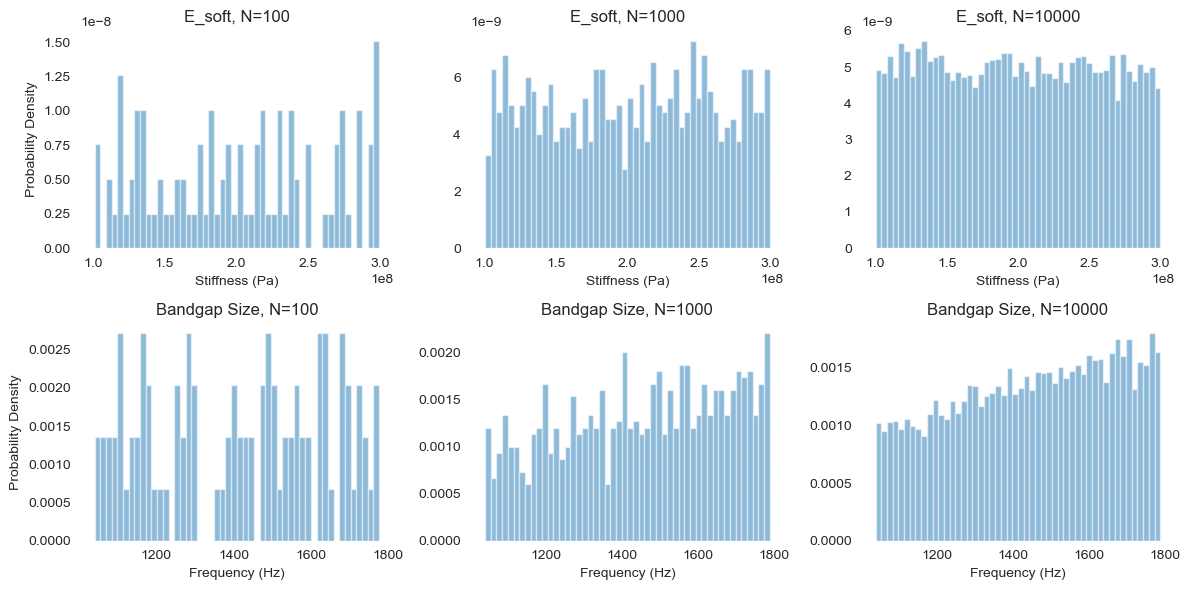
\includegraphics[width=\textwidth]{Figures/P_1d_input_E_soft_q_bgs_trio_hist.png}	
%         \caption{Histograms of 100, 1000, and 10000 randomly sampled soft material stiffness (top row) and corresponding computed bandgap sizes (bottom row).}
% 	\label{fig:1d_input_E_soft_q_bgs_trio_hist}%
% \end{figure}

\begin{figure}[H]
    \centering
    \begin{subfigure}{0.3\textwidth}
        \centering
        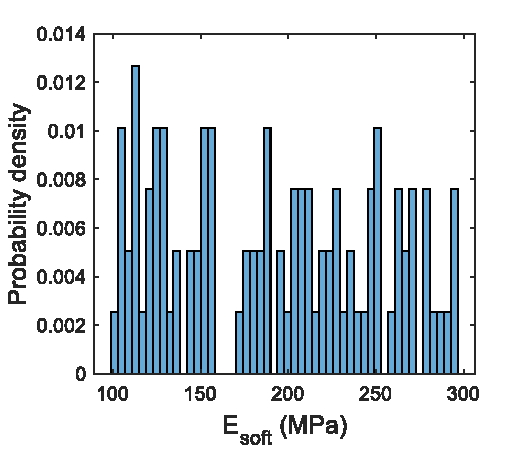
\includegraphics[width=\textwidth]{FinalFigures/P_1d_input_E_soft_q_bgs_trio_hist_a.pdf}
        \caption{}
        \label{fig:subfig-1}
    \end{subfigure}\quad
    \begin{subfigure}{0.3\textwidth}
        \centering
        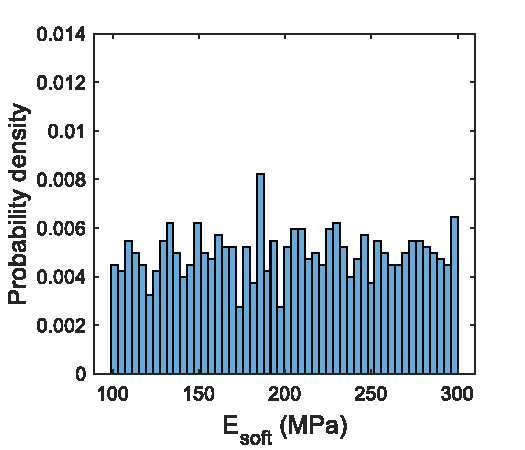
\includegraphics[width=\textwidth]{FinalFigures/P_1d_input_E_soft_q_bgs_trio_hist_b.pdf}
        \caption{}
        \label{fig:subfig-2}
    \end{subfigure}\quad
    \begin{subfigure}{0.3\textwidth}
        \centering
        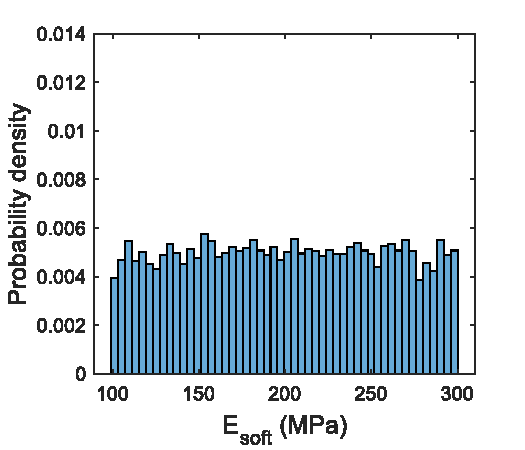
\includegraphics[width=\textwidth]{FinalFigures/P_1d_input_E_soft_q_bgs_trio_hist_c.pdf}
        \caption{}
        \label{fig:subfig-3}
    \end{subfigure}
        
    \begin{subfigure}{0.3\textwidth}
        \centering
        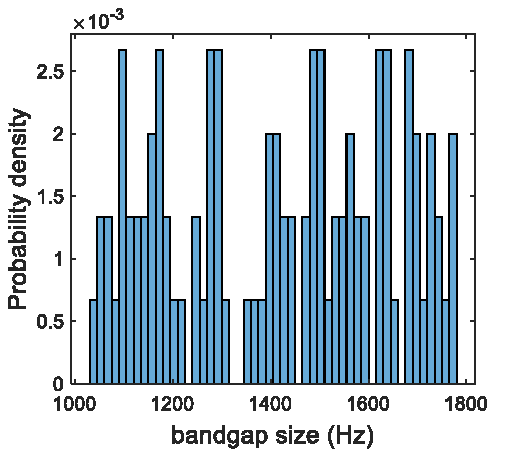
\includegraphics[width=\textwidth]{FinalFigures/P_1d_input_E_soft_q_bgs_trio_hist_d.pdf}
        \caption{}
        \label{fig:subfig-4}
    \end{subfigure}\quad
    \begin{subfigure}{0.3\textwidth}
        \centering
        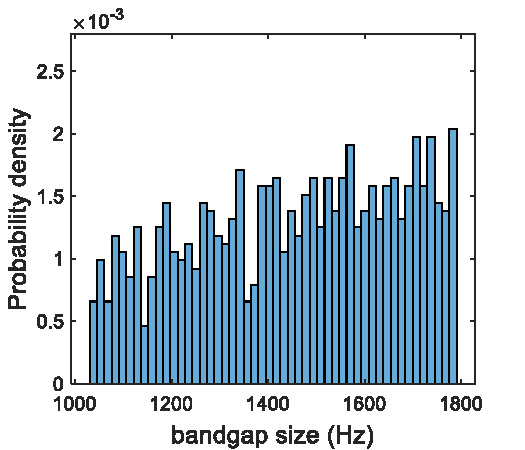
\includegraphics[width=\textwidth]{FinalFigures/P_1d_input_E_soft_q_bgs_trio_hist_e.pdf}
        \caption{}
        \label{fig:subfig-5}
    \end{subfigure}\quad
    \begin{subfigure}{0.3\textwidth}
        \centering
        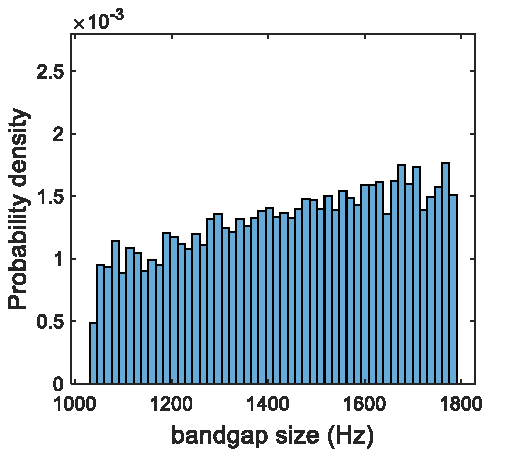
\includegraphics[width=\textwidth]{FinalFigures/P_1d_input_E_soft_q_bgs_trio_hist_f.pdf}
        \caption{}
        \label{fig:subfig-6}
    \end{subfigure}    
    \caption{Histograms of Young's modulus of soft material for a) 100, b) 1000, and c) 10000 samples and corresponding FE computed bandgap sizes for d) 100, e) 1000, and f) 10000 samples.}
    \label{fig:1d_input_E_soft_q_bgs_trio_hist}
\end{figure}

For the quadrature rule sampling strategy, we will look at orders \(N = 2 \text{ to } 5\), which corresponds in the 1D case (\(m=1\)) to a number of points \(n = (N+1)^m = 3 \text{ to } 6\).
% \begin{figure}[h]
% 	\centering
% 	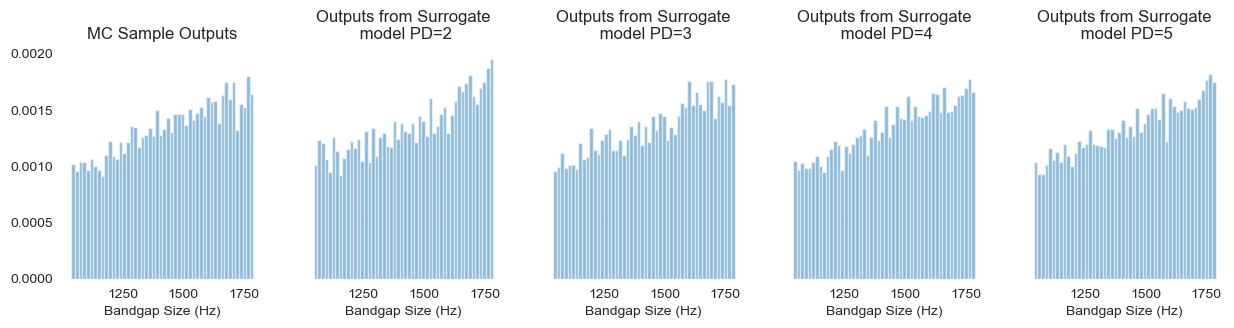
\includegraphics[width=\textwidth]{Figures/1d_input_E_soft_q_bgs_quinto_hist.png}	
%         \caption{Histograms of 10000 output samples drawn from finite element on Monte Carlo samples, and PCE surrogate models fitted to 3,4,5, and 6 quadrature rule points respectively.}
% 	\label{fig:1d_input_E_soft_q_bgs_quinto_hist}%
% \end{figure}

\begin{figure}[H]
    \centering
    \begin{subfigure}{0.32\textwidth}
        \centering
        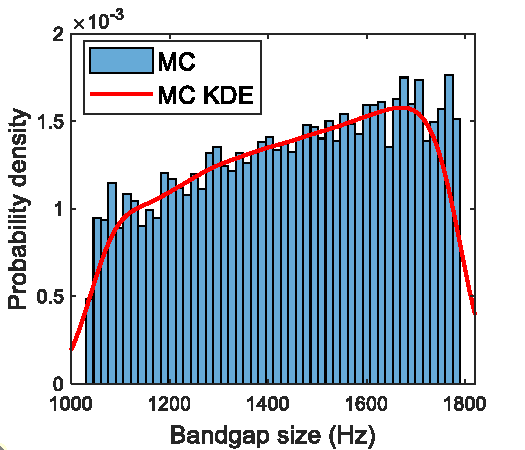
\includegraphics[width=\textwidth]{FinalFigures/1d_input_E_soft_q_bgs_quinto_hist_a.pdf}
        \caption{}
        \label{fig:subfig-1}
    \end{subfigure}
    \begin{subfigure}{0.32\textwidth}
        \centering
        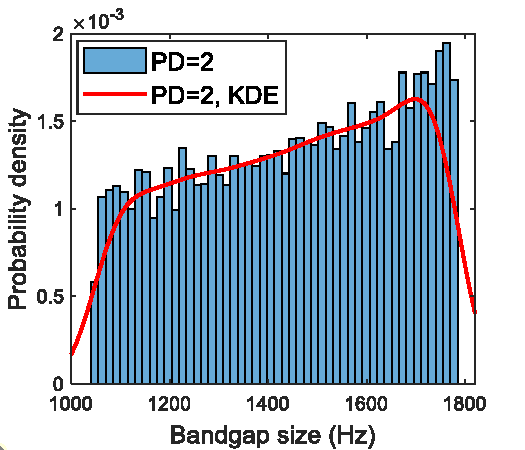
\includegraphics[width=\textwidth]{FinalFigures/1d_input_E_soft_q_bgs_quinto_hist_b.pdf}
        \caption{}
        \label{fig:subfig-2}
    \end{subfigure}
    
    %\vspace{0.5cm}
    
    \begin{subfigure}{0.32\textwidth}
        \centering
        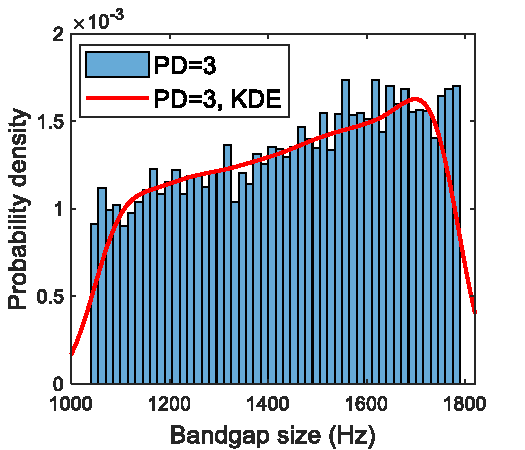
\includegraphics[width=\textwidth]{FinalFigures/1d_input_E_soft_q_bgs_quinto_hist_c.pdf}
        \caption{}
        \label{fig:subfig-3}
    \end{subfigure}
    \begin{subfigure}{0.32\textwidth}
        \centering
        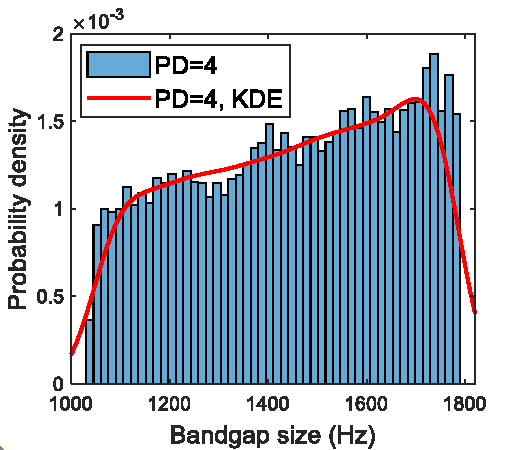
\includegraphics[width=\textwidth]{FinalFigures/1d_input_E_soft_q_bgs_quinto_hist_d.pdf}
        \caption{}
        \label{fig:subfig-4}
    \end{subfigure}
    \begin{subfigure}{0.32\textwidth}
        \centering
        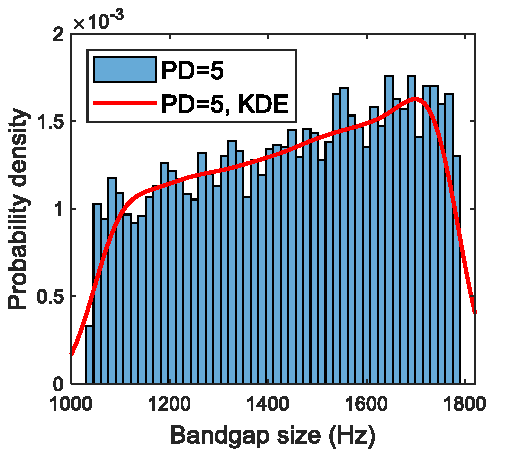
\includegraphics[width=\textwidth]{FinalFigures/1d_input_E_soft_q_bgs_quinto_hist_e.pdf}
        \caption{}
        \label{fig:subfig-5}
    \end{subfigure}    
    \caption{Histograms of a) 10000 FE computed outputs on MC samples, compared to PCE surrogate models fitted to b) 3, c) 4, d) 5, and e) 6 quadrature rule samples.}
    \label{fig:1d_input_E_soft_q_bgs_quinto_hist}
\end{figure}

From the results in \cref{fig:1d_input_E_soft_q_bgs_quinto_hist}, we can see that at orders 2 and above, the surrogate model output distribution is virtually indistinguishable from the true output probability density. This is a remarkable result that demonstrates with just 3 to 6 samples (and appropriate weights), we are able to capture the underlying probability distribution governing these samples. 

%%%%%%%%%%%%%%%%%%%%%%%%%%%%%%%%%%%%%%%%%%%%%%%%%%%%%%%%%%%%%%%%%%%%%%%%%%%%%%%%%%%%%%%%%%%%%%%%%%%%%%%%%%%%%%%%%%%
\subsection{Geometry Encoding Schema}
In general, there are three types of approaches to encoding geometries, each of which suffer from different advantages and disadvantages. The brute force way of explicitly defining each pixel of a given geometry is the most straight forward, offers the most control, but is computationally very costly, with input dimensionality scaling quadratically (in 2D) with resolution, which when coupled with the exponential scaling of sampling requirements with input dimensionality for UQ sampling strategies, renders only Monte Carlo sampling as an option for doing UQ on this encoding schema. 

A second class of approaches is to encode the geometry as a set of latent features, an approach that is popular in many machine learning and deep learning endeavors \citep{ChenWei2022}. This approach can be highly efficient, and theoretically can be the most efficient with appropriate regularization in the loss function penalizing redundant or unnecessary latent features. However, the main drawback of this approach is that often the number of latent features and their physical meaning is not interpretable. This also means it can be extremely difficult for technicians or engineers to examine samples in a realistic manufacturing scenario and ascribe probability distributions to each of the latent features, a step that is necessary to leverage the power of PCE and spectral projection. 

The final class of approaches are those like the algorithm detailed in methodology \Cref{subsubsec:m_geo}. These are interpretable encodings that rely on some symmetry or intuition of the physical world in order to reduce the set of all possible deformations to the set of those likely or interesting to a given problem. For our problem setup, it was the intuition of how such acoustic metamaterials would be manufactured that informed restricting geometric defects to occur at the edges. 

Our novel approach to encoding geometry defects allows geometry stochasticity to be captured in a one-dimensional, scale-invariant parameter``flip proportion", for UQ or statistical analysis. This encoding schema serves as a highly efficient default encoding schema which can be further refined by ``depth'' parameters which control how deep the defects can occur within the bulk geometry or ``skew'' parameters which bias the defects to occur in certain regions of the geometry. Such parameters were not needed however to demonstrate the utility of UQ techniques for the studies in this paper and so were not implemented. The concerns regarding the non-determinism of defective geometries with the same FP parameter were mitigated by studying the bandgap size and location variance of sample geometries with the same FP parameter, which was much smaller than the effects of material property variance, justifying the representation of possible defects with the pseudo-deterministic FP parameter. This also implies that in an infinite grid of unit cell geometries with different exact defects each, the combined effect of their defects will be small relative to material property stochasticity and be well represented by the FP parameter.

%%%%%%%%%%%%%%%%%%%%%%%%%%%%%%%%%%%%%%%%%%%%%%%%%%%%%%%%%%%%%%%%%%%%%%%%%%%%%%%%%%%%%%%%%%%%%%%%%%%%%%%%%%%%%%%%%%%
\subsection{Spectral projection \& PCE}
From the studies in \Cref{subsec:7D Gamma Input Space} and \Cref{subsec:7D Gaussian Input Space}, 
we found that all of the three spectral projection sampling strategies (namely, MC sampling, quadrature rule, and sparse grid) were able to capture the probability distribution of the 2D output space of bandgap size and location given a 7D input space of 6 material properties and a geometry defect parameter. We see the most extreme sample size savings for the sparse grid approach, which with \(\sim 15\) points, was able to capture fairly accurately the output probability distribution. The sparse grid approach however, despite working well for this application, may not work as well for output landscapes with many local features, which may be missed by the sparse grid points. Quadrature rule sampling, which returns a full grid instead of a sparse grid of points in the input space, is less likely to miss local features, but scales exponentially with input dimension and so is not computationally practical for much higher of a input space dimensionality than what is done in this paper's studies. Monte Carlo sampling paired with PCE is relatively less effective at lower dimensions, but because it does not scale directly with the input space dimensionality (although it can scale through indirect means, such as model complexity which typically increases with input dimensionality). For that same reason however, Monte Carlo outperforms at higher dimensions, slightly beating out quadrature rule in our studies at 100 points to achieve good fit over 128 points for the 1\textsuperscript{st} degree quadrature rule. As seen in \Cref{subsec:1D Uniform Input Space Study} however, in the 1D case, quadrature rule spectral projection dominates, requiring only a handful of samples (3-6) to faithfully capture the output probability distribution of a finite element model. These results are in line with prevailing wisdom about the different spectral projection sampling strategies. In general, spectral projection and PCE is a powerful tool for analysing acoustic metamaterial performance characteristics in the context of stochastic material properties or geometry and potentially of great practical use to characterizing manufacturing processes.
%%%%%%%%%%%%%%%%%%%%%%%%%%%%%%%%%%%%%%%%%%%%%%%%%%%%%%%%%%%%%%%%%%%%%%%%%%%%%%%%%%%%%%%%%%%%%%%%%%%%%%%%%%%%%%%%%%%

\section{Conclusions}
\label{sec:Conclusion}
%%%%%%%%%%%%%%%%%%%%%%%%%%%%%%%%%%%%%%%%%%%%%%%%%%%%%%%%%%%%%%%%%%%%%%%%%%%%%%%%%%%%%%%%%%%%%%%%%%%%%%%%%%%%%%%%%%%
In this paper, we applied the UQ techniques of representation through polynomial chaos expansions and propagation using spectral projections on three different scenarios to demonstrate the utility and generalizability of such techniques in capturing the probability distributions of performance characteristics given simultaneous stochasticity in up to seven input parameters.

From the three studies performed in this paper on different design geometries, material property distributions, and input space dimensionality, we find the sparse grid sampling strategy performs well when input space dimensionality is low, whereas quadrature rule performs well when input space dimensionality is high. Monte Carlo sampling strikes a balance, underperforming relative to the other two strategies in low dimensional input spaces but eventually becoming the most efficient method for very high dimension input spaces. These sampling strategies combined with PCE and spectral projection very accurately represented the effects of stochastic material input parameters with 10s to 100s of  samples for the 7D case, versus 1000s to 10000s for brute force sampling, and with less than 10 samples for the 1D case, compared to 100s of samples for brute force sampling. We can conclude that PCE and spectral projection are powerful UQ methods which can reduce sampling needs by orders of magnitude and generally applicable to capturing stochastic effects on metamaterial performance characteristics. 

The ``edge-pixel flip proportion'' method introduced used in this paper proved to be an effective schema for encoding geometry stochasticity. This method constrained the input dimensionality for representing geometry to just one dimension, while being scale invariant, physically meaningful, and realistic in representing real world defects. The pseudo-deterministic nature of this method, where the same FP parameter maps to multiple defect geometries, proved to be no issue for UQ because the metamaterial characteristics' variations for the same flip proportion parameter were orders of magnitude smaller than variations for different flip proportion parameters and for different material properties.

In a realistic manufacturing scenario, this drastic reduction \rev{(of several orders of magnitude) in sampling needs---which results from efficient geometry encoding and the use of appropriate UQ techniques---can allow for conservation of time and resources during the design and testing of metamaterials.} Such techniques therefore show great economic promise in industrial fabrication as well as academic experimentation, \rev{without requiring much startup cost to adopt in typical design cycles}. Further refinements can be explored in the sampling techniques, surrogate model construction methods, as well as how to encode more complex defects in geometries, to increase the utility of such methods and widen their applicability to other metamaterial or material design and manufacturing problems.

\section*{Declaration of Competing Interest}
The authors declare that they have no known competing financial interests or personal relationships that could have appeared to influence the work reported in this paper.

\section*{CRediT authorship contribution statement}
\textbf{Han Zhang:} Conceptualization, Methodology, Software, Validation, Formal Analysis, Investigation, Data Curation, Writing - Original Draft, Writing - Review \& Editing, Visualization. \textbf{Rayehe Karimi Mahabadi:} Conceptualization, Writing - Original Draft, Writing - Review \& Editing, Visualization, Supervision. \textbf{Cynthia Rudin:} Writing - Review and Editing, Funding Acquisition. \textbf{Johann Guilleminot:} Conceptualization, Validation, Formal Analysis, Writing - Original Draft, Writing - Review \& Editing. \textbf{L. Catherine Brinson:} Conceptualization, Methodology, Resources, Writing - Review \& Editing, Supervision, Project Administration, Funding Acquisition.

\section*{Data availability}
The code and data in this article
can be found at this GitHub repository:
\url{https://github.com/trutheresy/UQ-2D-Metamaterials}.

\section*{Acknowledgements}
The authors gratefully acknowledge funding from the U.S. Department of Energy under Grant No. DE-SC0021358 and the National Science Foundation under Grant No. DGE-2022040. Special thanks to Alexander C. Ogren of the California Institute of Technology for providing the finite element analysis code which served as the ground truth model to generate samples from and compare surrogate model performance with. 

%% The Appendices part is started with the command \appendix;
%% appendix sections are then done as normal sections
%\appendix
%\section{Supplementary Figures}
%\subsection{7D Gamma \& Beta Distribution Experiment}

%\subsection{7D Gaussian Distribution Experiment}
%% \label{}

%\section{Appendix title 2}
%% \label{}

%% If you have bibdatabase file and want bibtex to generate the
%% bibitems, please use
%%
\bibliographystyle{elsarticle-num}
%\bibliographystyle{plain} 
\bibliography{references}
%\todo{Add some references for metamaterials, or UQ}
%% else use the following coding to input the bibitems directly in the
%% TeX file.

%%\begin{thebibliography}{00}

%% \bibitem[Author(year)]{label}
%% For example:

%% \bibitem[Aladro et al.(2015)]{Aladro15} Aladro, R., Martín, S., Riquelme, D., et al. 2015, \aas, 579, A101


%%\end{thebibliography}

\end{document}

\endinput
%%
%% End of file `elsarticle-template-harv.tex'.
